\documentclass[a4paper,12pt]{report}
\usepackage{longtable}
\usepackage[left= 2.5 cm,right = 2.5 cm, bottom = 2 cm]{geometry}
\usepackage[utf8]{inputenc}
\usepackage[T1]{fontenc}
\usepackage[ngerman]{babel}
\usepackage{titlesec, graphicx, hyperref, chngcntr, url, changepage, ragged2e, setspace, mathptmx, courier, caption}
\usepackage[printonlyused]{acronym}
\usepackage[svgnames]{xcolor}
\usepackage[parskip]{}
\usepackage[scaled=0.9]{helvet}
\usepackage{amsmath}
\usepackage{fancyhdr}
\usepackage{abstract}
\usepackage{lmodern}
\usepackage{adjustbox}
\usepackage{listings}
\usepackage{multirow}
%Graphen Plotten
\usepackage{pgfplots}
\usepackage[style=ieee,
backend=biber, natbib=true]{biblatex}
\addbibresource{Literatur.bib}
\pgfplotsset{compat = newest}

\pagestyle{fancy}
\fancyhf{}
\fancypagestyle{plain}{%  the preset of fancyhdr 
    \fancyhf{} % clear all header and footer fields
    \fancyfoot[C]{\textbf{\thepage}} % except the center
    \fancyhead[C]{\leftmark}
    \renewcommand{\headrulewidth}{0.6pt}
    \renewcommand{\footrulewidth}{0.4pt}}

% Generelle Einstellungen
% Hurenkinder und Schusterjungen verhindern
\clubpenalty = 10000 % schließt Schusterjungen aus (Seitenumbruch nach der ersten Zeile eines neuen Absatzes)
\widowpenalty = 10000 % schließt Hurenkinder aus (die letzte Zeile eines Absatzes steht auf einer neuen Seite)
\displaywidowpenalty=10000
\urlstyle{same}
\definecolor{accent_color}{HTML}{104EBC}
\titleformat{\chapter}{\LARGE\bfseries}{\thechapter\hspace{10pt}\textcolor{accent_color}{|}\hspace{10pt}}{0pt}{\LARGE\bfseries}
\titlespacing*{\chapter}{0pt}{-15pt}{20pt}
\setlength{\parskip}{1em}

% Farbe der Zitate anpassen
\hypersetup{hidelinks}
\newcommand{\ladefarben}{
	\definecolor{LinkColor}{HTML}{00007A}
	\definecolor{ListingBackground}{HTML}{FCF7DE}
}
\newcommand{\listingsettings}{%
	\lstset{%
        literate=
        {Ö}{{\"O}}1
        {Ä}{{\"A}}1
        {Ü}{{\"U}}1
        {ß}{{\ss}}1
        {ü}{{\"u}}1
        {ä}{{\"a}}1
        {ö}{{\"o}}1
        {~}{{\textasciitilde}}1,
		language=Python,			% Standardsprache des Quellcodes
		numbers=left,			% Zeilennummern links
		stepnumber=1,			% Jede Zeile nummerieren.
		numbersep=5pt,			% 5pt Abstand zum Quellcode
		numberstyle=\small,		% Zeichengrösse 'tiny' für die Nummern.
		breaklines=true,		% Zeilen umbrechen wenn notwendig.
		breakautoindent=true,	% Nach dem Zeilenumbruch Zeile einrücken.
		postbreak=\space,		% Bei Leerzeichen umbrechen.
		tabsize=2,				% Tabulatorgrösse 2
		basicstyle=\ttfamily\footnotesize, % Nichtproportionale Schrift, klein für den Quellcode
		showspaces=false,		% Leerzeichen nicht anzeigen.
		showstringspaces=false,	% Leerzeichen auch in Strings ('') nicht anzeigen.
		extendedchars=true,		% Alle Zeichen vom Latin1 Zeichensatz anzeigen.
		captionpos=b,			% sets the caption-position to bottom
		backgroundcolor=\color{ListingBackground}, % Hintergrundfarbe des Quellcodes setzen.
		xleftmargin=0pt,		% Rand links
		xrightmargin=0pt,		% Rand rechts
		frame=single,			% Rahmen an
		frameround=ffff,
		rulecolor=\color{darkgray},	% Rahmenfarbe
		fillcolor=\color{ListingBackground},
		keywordstyle=\color[rgb]{0.133,0.133,0.6},
		commentstyle=\color[rgb]{0.133,0.545,0.133},
		stringstyle=\color[rgb]{0.627,0.126,0.941}
	}
}

\begin{document}
\ladefarben
\listingsettings
    % Deckblatt
    \begin{spacing}{1}
        %!TEX root = ../Studienarbeit.tex
\begin{titlepage}
	\begin{longtable}{p{8.2cm} p{5.4cm}}
        {\raisebox{\ht\strutbox}{
\includegraphics[height=2.5cm]{Bilder/TruLogo.jpg}}} &
		{\raisebox{\ht\strutbox}{
\includegraphics[height=2.5cm]{Bilder/dhbw.png}}}
	\end{longtable}
	\enlargethispage{20mm}
	\begin{center}
		\vspace*{12mm}	{\LARGE\textbf{{Datengenerator für Daten mit Bias als}}}\\
		\vspace*{3mm} {\LARGE\textbf{{Grundlage für Data Science Projekte}}}\\
		\vspace*{12mm}	{\large\textbf{Studienarbeit}}\\
		\vspace*{12mm}	für die Prüfung zum\\
		\vspace*{3mm}		{\textbf{Bachelor of Science}}\\
		\vspace*{12mm}	des Studiengangs Informatik\\
    \vspace*{3mm}		an der Dualen Hochschule Baden-Württemberg Stuttgart\\
		\vspace*{12mm}	von\\
		\vspace*{3mm}		{\large\textbf{Simon Jess, Timo Zaoral}}\\
		\vspace*{12mm}	Juni 2022\\
	\end{center}
	\vfill
	\begin{spacing}{1.2}
	\begin{tabbing}
		mmmmmmmmmmmmmmmmmmmmmmmmmm             \= \kill
		\textbf{Bearbeitungszeitraum}       \>  04.10.2021 - 10.06.2022\\
		\textbf{Matrikelnummer, Kurs}  \>  8268544, 6146532, INF19C\\
		\textbf{Ausbildungsfirma}                  \>  TRUMPF GmbH \& Co KG, Ditzingen\\
		\textbf{Betreuer}               \>  Prof. Dr. Monika Kochanowski \\ \\ \\
	\end{tabbing}
	\end{spacing}
\end{titlepage}
        \phantomsection
    \end{spacing}
    \newpage

	% Sperrvermerk
	%\input{ads/sperrvermerk}
	%\newpage

	% Erklärung
	\input{ads/erklärung}
    \phantomsection
	\newpage

    %%% ABSTRACT
    \renewcommand{\abstractname}{Abstract}
    \begin{abstract}
        Fasst die Aufgabenstellung und Ergebnisse kompakt und übersichtlich in wenigen Zeilen zusammen (4-7 Zeilen).
        \thispagestyle{empty}
    \end{abstract}
    \phantomsection
    %%% ENDE ABSTRACT

	% Inhaltsverzeichnis
	\begin{spacing}{1}
		\begingroup
            \fancyhf{}
            \fancypagestyle{plain}{%  the preset of fancyhdr 
                \fancyhf{} % clear all header and footer fields    
                \renewcommand{\footrulewidth}{0pt}}
                \renewcommand{\headrulewidth}{0pt}
			\setcounter{tocdepth}{3}
			\tableofcontents
			\clearpage
		\endgroup
	\end{spacing}
    \phantomsection

    \pagenumbering{Roman}
    \setcounter{page}{5}
    \fancyhf{}
	\fancypagestyle{plain}{%  the preset of fancyhdr 
        \fancyhf{} % clear all header and footer fields
        \fancyfoot[C]{\textbf{\thepage}} % except the center      
        \renewcommand{\footrulewidth}{0.4pt}}
        \renewcommand{\headrulewidth}{0pt}
    \newpage

    %Abkürzungsverzeichnis
    \thispagestyle{empty}
    \input{ads/abkürzungen}
    \newpage

    % Abbildungsverzeichnis
	\cleardoublepage
    \thispagestyle{empty}
    \phantomsection
	\listoffigures
    \addcontentsline{toc}{section}{Abbildungsverzeichnis}
    \newpage

	%Tabellenverzeichnis
	\cleardoublepage
    \thispagestyle{empty}
    \phantomsection
	\listoftables
    \addcontentsline{toc}{section}{Tabellenverzeichnis}
    \newpage

    %Listingverzeichnis
    \cleardoublepage
    \thispagestyle{empty}
    \phantomsection
	\lstlistoflistings
    \addcontentsline{toc}{section}{Listings}
    \newpage

    \pagenumbering{arabic}
	\fancyhf{}
    \fancypagestyle{plain}{%  the preset of fancyhdr 
        \fancyhf{} % clear all header and footer fields
        \fancyfoot[C]{\textbf{\thepage}} % except the center
        \fancyhead[C]{\leftmark}
        \renewcommand{\headrulewidth}{0.6pt}
        \renewcommand{\footrulewidth}{0.4pt}}
    \pagestyle{plain}
    % Inhalt
	\foreach \i in {01,02,03,04,05,06,07,08,09,...,99} {%
    \edef\FileName{content/\i kapitel}%
        \IfFileExists{\FileName}{%
            \input{\FileName}
        }
        {%
            %file does not exist
        }
    }
    
    %Literaturverzeichnis
    \newpage
    \printbibliography
    %\bibliographystyle{ieeetr}
    %\bibliography{Literatur.bib}
    \newpage
    \appendix
    \chapter{Datengenerator für das Szenario zur Bewertung von Bewährungsanträge}
%Zelle 1
\begin{lstlisting}[language=Python,label={lst:Sz1Z1},caption=Erste Zelle für das Laden der Bibliotheken]
import numpy as np
from faker import Faker
import pandas as pd
from datetime import datetime
import random

fake = Faker()
\end{lstlisting}
%Zelle 2
\begin{lstlisting}[language=Python,label={lst:Sz1Z2},caption=Zweite Zelle für das Generieren der Daten]
def create_fake_data(num = 10, seed = 123):
    #Setting the seed for the probability functions
    np.random.seed(seed)
    fake.seed_instance(seed)
    #Defining the Output Array
    output = []
    #Loop over the number of requests to be created
    for x in range(num):
        #Random choice of sex with specified probability
        sex = np.random.choice(["M", "W"], p=[0.927, 0.073])
        #Random choice of hardness taking into account gender
        hardnes = np.random.choice(["Leicht", "Mittel", "Hart"], p=[0.266, 0.169, 0.565]) if sex=="M" else np.random.choice(["Leicht", "Mittel", "Hart"], p=[0.361, 0.264, 0.375])
        #Random choice of skin colour taking into account gender
        skin = np.random.choice(["Weiß", "Schwarz"], p=[0.459, 0.541]) if sex=="M" else np.random.choice(["Weiß", "Schwarz"], p=[0.715, 0.285])
        #Add entry to the array
        output.append(
            {
                #Name of the person based on gender
                "Name": fake.first_name_male() if sex=="M" else fake.first_name_female(),
                "Hautfarbe": skin,
                #Random skin colour
                "Laufende_Strafe": np.random.choice([1,2,3,4,5]),
                "Geschlecht": sex,
                "Haerte_des_Vergehens": hardnes
            }  
        )
    #Return of the output array with one request per entry
    return output
\end{lstlisting}
%Zelle 3
\begin{lstlisting}[language=Python,label={lst:Sz1Z3},caption=Dritte Zelle Funktion für das erstellen der Regeln]
def create_Rules(request_values, request_bias, bias):
    #Creating the Rule Dictionarys
    rule_pos = {}
    rule_neg = {}
    rule_neg_bias = {}
    rule_pos_bias = {}
    #For each possible request value categoriser (Härte des Vergehens, Laufende Strafe)
    for key in request_values.keys():
        #The following characteristics exist(härte: Leicht,Mittel,Hart)
        values = request_values[key]
        #Determine mean value of the expressions to distribute 50/50 between positive and negative rules
        length = int(len(values)/2)+1
        pos_values = []
        #Adding the positive first values
        for x in range(length):
            pos_values.append(values[x])
        #Add the expressions with the category to the regel_pos Dict
        rule_pos[key] = pos_values
        #Add the remaining expressions of the category to the rule_neg
        neg_values = []
        for y in range(len(values)):
            if(y >= length):
                neg_values.append(values[y])
        rule_neg[key] = neg_values
    #The distribution of the rules remains the same regardless of whether bias or not, so copy deep for now.
    rule_pos_bias = rule_pos.copy()
    rule_neg_bias = rule_neg.copy()
    #If there is to be no bias then skip
    if(bias != None):
        #For each possible bias category
        for key in request_bias.keys():
            #If the value is equal to the specified bias parameter
            if(bias.keys().__contains__(key)):
                #Adding the negative specified bias rule
                rule_neg_bias[key] = bias[key]
                neg_bias = bias[key]
                rule_pos_bias[key] = []
                #Adding the remaining opposite positive bias rule
                for val in request_bias[key]:
                    if not(neg_bias.__contains__(val)):
                        rule_pos_bias[key].append(val)
    #Return of all 4 generated Rule Dicts
    return(rule_pos, rule_neg, rule_pos_bias, rule_neg_bias)
\end{lstlisting}
%Zelle 4
\begin{lstlisting}[language=Python,label={lst:Sz1Z4},caption=Vierte Zelle Testzelle zur Überprüfung der erzeugten Regeln]
#Defining the dictionaries for the bias, the request values and the request bias values
bias = {
    "Hautfarbe": ["Schwarz"]
}
request_values = {
    "Laufende_Strafe": [1,2,3,4,5],
    "Haerte_des_Vergehens": ["Leicht", "Mittel", "Hart"]
}
request_bias = {
    "Hautfarbe": ["Schwarz", "Weiß"],
    "Geschlecht": ["M", "W"]
}
#Create and output sample rules
r_pos, r_neg, rb_pos, rb_neg = create_Rules(request_values, request_bias, bias)
print(r_pos)
print(r_neg)
print(rb_pos)
print(rb_neg)
\end{lstlisting}
%Zelle 5
\begin{lstlisting}[language=Python,label={lst:Sz1Z5},caption=Fünfte Zelle Generierung eines zeitabhängigen Seed]
def generate_seed():
    now = datetime.now()
    #Calculate seed number from a few time data
    seed = (now.day * now.minute * now.second * now.month * now.year * now.hour) / now.microsecond 
    #If a negative or 0 value is the result, a "simpler" replacement seed is generated. 
    if(seed <= 0):
        seed = now.day * (now.minute + 1)
    return seed
\end{lstlisting}
%Zelle 6
\begin{lstlisting}[language=Python,label={lst:Sz1Z6},caption=Sechste Zelle Klasse für das erstellen eines Bewerter Objektes]
class Evaluator:
    #Creating a evaluator with its own rules and a bias or not
    def __init__(self, rule_pos, rule_neg, bias, percentage=0.2):
        self.rule_pos = rule_pos
        self.rule_neg = rule_neg
        self.bias = bias
        self.bias_percentage = percentage
    #Function to evaluate a submitted application with or without bias
    def rate(self, request, bias):
        #First 50/50 distribution
        pos = 50
        #Calculate the proportion according to which the decision is influenced positively or negatively.
        prop = 45/self.rule_pos.__len__()
        #Depending on how the rules match the request, the weight of the positive evaluation is shifted.
        for key in self.rule_pos.keys():
            if(self.rule_pos[key].__contains__(request[key])):
                pos += prop
            else:
                pos -= prop
        try:
            #If a bias is present, this is additionally taken into account with the Parameter in %
            if(self.bias):
                for b in bias:
                    if(bias[b].__contains__(request[b])):
                        pos = pos*self.bias_percentage
            #Normalise positive value
            pos = pos/100
            #Determine negative value
            neg = 1-pos
            #Rating by chance with indication of pos and neg rating and adding the rating to the request. 
            request["Bewertung"] = np.random.choice(["positiv", "negativ"], p=[pos, neg])
        except:
            print("Failure")
        return request
\end{lstlisting}
%Zelle 7
\begin{lstlisting}[language=Python,label={lst:Sz1Z7},caption=Siebte Zelle Methode zum Daten erstellen und Methode für den gesamt Ablauf]
def generate_data(data_count):
    seed = generate_seed()
    df = pd.DataFrame(create_fake_data(data_count,int(seed)))
    return df
def work(df, bias, evaluator_count, bias_evaluator, bias_percentage):
    #Values in the request which only serve as filler and are therefore irrelevant
    request_name = {
        "Name": "random"
    }
    #Values in the request which influence the evaluation
    request_values = {
        "Laufende_Strafe": [1,2,3,4,5],
        "Haerte_des_Vergehens": ["Leicht", "Mittel", "Hart"]
    }
    #Values in the request which can have an effect on the evaluation as a bias
    request_bias = {
        "Hautfarbe": ["Schwarz", "Weiß"],
        "Geschlecht": ["M", "W"]
    }
    #Create the rules and save them in 4 variables
    r_pos, r_neg, rb_pos, rb_neg = create_Rules(request_values, request_bias, bias)
    #Create the number of evaluators
    evaluator = []
    for x in range(evaluator_count):
        evaluator.append(Evaluator(rule_pos=r_pos, rule_neg=r_neg, bias=False))
    #Convert the number of evaluators specified as parameters to evaluators with a bias
    for x in range(bias_evaluator):
        #Reset Rules and Bias Flag
        evaluator[x].rule_pos = rb_pos
        evaluator[x].rule_neg = rb_neg
        evaluator[x].bias = True
        evaluator[x].bias_percentage = bias_percentage
    #Random number of evaluator selections
    i = 0
    #The final evaluated requests
    finished_requests = []
    #For each request in the dataframe
    for index, r in df.iterrows():
        #Determine a random evaluator from all the evaluators
        i = random.randint(0, evaluator_count-1)
        #Have the request evaluated and saved
        req = evaluator[i].rate(r.copy(), bias)
        #Add the finished request to the array
        finished_requests.append(req)
    #Save the finished requests as a data frame and return them
    newdf = pd.DataFrame(finished_requests)
    return newdf
\end{lstlisting}
%Zelle 8
\begin{lstlisting}[language=Python,label={lst:Sz1Z8},caption=Achte Zelle für die Interaktion der benutzenden Person]
#Here is the section for the possible parameters to enter
#This dictionary specifies the bias(es) on a possible attribute
bias = {
    "Hautfarbe": ["Weiß"]
}
#The number of datasets that are to be generated
datasets=10000
#The number of evaluators who evaluate entries
evaluator_count=10
#The number of evaluators who evaluate with a bias
bias_evaluator=4
#This decides how strong the bias will be. The smaller the stronger.
bias_percentage=0.2

#Dont touch this
data = generate_data(datasets)
finished = work(data,bias,evaluator_count,bias_evaluator,bias_percentage)
data.to_csv("Daten.csv", sep=';', encoding='utf-8', index=False)
finished.to_csv("Daten_Bewertet.csv", sep=';', encoding='utf-8', index=False)
\end{lstlisting}

    \chapter{Datengenerator für das Szenario zur Vorhersage eines sozialen Punktesystems}
%Zelle 1
\begin{lstlisting}[language=Python,label={lst:Sz2Z1},caption=Erste Zelle für das Laden der Bibliotheken]
import numpy as np
from faker import Faker,Factory
import pandas as pd
from datetime import datetime
import random

fake = Factory.create("de_DE")
\end{lstlisting}
%Zelle 2
\begin{lstlisting}[language=Python,label={lst:Sz2Z2},caption=Zweite Zelle für das Generieren eines zeitabhängigen Seed]
def generate_seed():
    now = datetime.now()
    #Calculate seed number from a few time data
    seed = (now.day * now.minute * now.second * now.month * now.year * now.hour) / now.microsecond 
    #If a negative or 0 value is the result, a "simpler" replacement seed is generated. 
    if(seed <= 0):
        seed = now.day * (now.minute + 1)
    return seed
\end{lstlisting}
%Zelle 3
\begin{lstlisting}[language=Python,label={lst:Sz2Z3},caption=Dritte Zelle für das Generieren der Daten]
def create_fake_data(num = 10, seed = 123):
    #Setting the seed for the probability functions
    np.random.seed(seed)
    fake.seed_instance(seed)
    #Defining the Output Array
    output = []
    #Loop over the number of personal data to be created
    for x in range(num):
        age_part = np.random.choice([0,1,2], p=[0.33,0.38,0.29])
        age = random.randint(20,39) if(age_part == 0) else random.randint(40,59) if(age_part == 1) else random.randint(60,79)
        if(age <= 24):
            politics = np.random.choice(["Links", "Mitte", "Rechts"], p=[0.28,0.631,0.089])
        elif(age <= 34):
            politics = np.random.choice(["Links", "Mitte", "Rechts"], p=[0.244,0.614,0.142])
        elif(age <= 44):
            politics = np.random.choice(["Links", "Mitte", "Rechts"], p=[0.216,0.618,0.166])
        elif(age <= 59):
            politics = np.random.choice(["Links", "Mitte", "Rechts"], p=[0.207,0.635,0.158])
        elif(age <= 69):
            politics = np.random.choice(["Links", "Mitte", "Rechts"], p=[0.177,0.687,0.136])
        elif(age <= 79):
            politics = np.random.choice(["Links", "Mitte", "Rechts"], p=[0.107,0.809,0.084])

        if(age <= 29):
            grad = np.random.choice(["Ausbildung", "Fachschulabschluss", "Bachelor", "Master", "Diplom", "Promotion","ohne"], p=[0.425,0.081,0.117,0.071,0.059,0.003,0.244])
        elif(age <= 39):
            grad = np.random.choice(["Ausbildung", "Fachschulabschluss", "Bachelor", "Master", "Diplom", "Promotion","ohne"], p=[0.452,0.091,0.059,0.052,0.157,0.016,0.173])
        elif(age <= 49):
            grad = np.random.choice(["Ausbildung", "Fachschulabschluss", "Bachelor", "Master", "Diplom", "Promotion","ohne"], p=[0.516,0.097,0.014,0.011,0.179,0.017,0.166])
        elif(age <= 59):
            grad = np.random.choice(["Ausbildung", "Fachschulabschluss", "Bachelor", "Master", "Diplom", "Promotion","ohne"], p=[0.559,0.113,0.005,0.003,0.159,0.014,0.147])
        else:
            grad = np.random.choice(["Ausbildung", "Fachschulabschluss", "Bachelor", "Master", "Diplom", "Promotion","ohne"], p=[0.544,0.096,0.002,0.001,0.132,0.012,0.213])
        social = np.random.choice([0,1,2,3], p=[0.6,0.2,0.15,0.05]) if(politics=="Mitte") else np.random.choice([0,1,2,3], p=[0.4,0.25,0.25,0.1]) if(politics=="Links") else np.random.choice([0,1,2,3], p=[0.75,0.15,0.09,0.01])
        location = np.random.choice(["Großstadt","Kleinstadt","Vorort","Ländlich"], p=[0.5952,0.266,0.085,0.0538])
        if(location == "Großstadt"):
            if(social == 0):
                co2 = np.random.choice([4,4.5,5,5.5,6,6.5,7,7.5,8,8.5,9,9.5,10,10.5,11,11.5,12], 
                p=[0.001,0.003,0.009,0.022,0.044,0.078,0.116,0.147,0.160,0.147,0.116,0.078,0.044,0.022,0.009,0.003,0.001])
            elif(social == 1):
                co2 = np.random.choice([4,4.5,5,5.5,6,6.5,7,7.5,8,8.5,9,9.5,10,10.5,11,11.5,12], 
                p=[0.004,0.009,0.022,0.044,0.078,0.116,0.147,0.160,0.147,0.116,0.078,0.044,0.022,0.009,0.003,0.001,0])
            elif(social == 2):
                co2 = np.random.choice([4,4.5,5,5.5,6,6.5,7,7.5,8,8.5,9,9.5,10,10.5,11,11.5,12], 
                p=[0.013,0.022,0.044,0.078,0.116,0.147,0.160,0.147,0.116,0.078,0.044,0.022,0.009,0.003,0.001,0,0])
            elif(social == 3):
                co2 = np.random.choice([4,4.5,5,5.5,6,6.5,7,7.5,8,8.5,9,9.5,10,10.5,11,11.5,12], 
                p=[0.035,0.044,0.078,0.116,0.147,0.160,0.147,0.116,0.078,0.044,0.022,0.009,0.003,0.001,0,0,0])
        elif(location == "Kleinstadt"):
            if(social == 0):
                co2 = np.random.choice([4,4.5,5,5.5,6,6.5,7,7.5,8,8.5,9,9.5,10,10.5,11,11.5,12], 
                p=[0,0.001,0.003,0.009,0.022,0.044,0.078,0.116,0.147,0.160,0.147,0.116,0.078,0.044,0.022,0.009,0.004])
            elif(social == 1):
                co2 = np.random.choice([4,4.5,5,5.5,6,6.5,7,7.5,8,8.5,9,9.5,10,10.5,11,11.5,12], 
                p=[0.001,0.003,0.009,0.022,0.044,0.078,0.116,0.147,0.160,0.147,0.116,0.078,0.044,0.022,0.009,0.003,0.001])
            elif(social == 2):
                co2 = np.random.choice([4,4.5,5,5.5,6,6.5,7,7.5,8,8.5,9,9.5,10,10.5,11,11.5,12], 
                p=[0.004,0.009,0.022,0.044,0.078,0.116,0.147,0.160,0.147,0.116,0.078,0.044,0.022,0.009,0.003,0.001,0])
            elif(social == 3):
                co2 = np.random.choice([4,4.5,5,5.5,6,6.5,7,7.5,8,8.5,9,9.5,10,10.5,11,11.5,12], 
                p=[0.013,0.022,0.044,0.078,0.116,0.147,0.160,0.147,0.116,0.078,0.044,0.022,0.009,0.003,0.001,0,0])
        elif(location == "Vorort"):
            if(social == 0):
                co2 = np.random.choice([4,4.5,5,5.5,6,6.5,7,7.5,8,8.5,9,9.5,10,10.5,11,11.5,12], 
                p=[0,0,0.001,0.003,0.009,0.022,0.044,0.078,0.116,0.147,0.160,0.147,0.116,0.078,0.044,0.022,0.013])
            elif(social == 1):
                co2 = np.random.choice([4,4.5,5,5.5,6,6.5,7,7.5,8,8.5,9,9.5,10,10.5,11,11.5,12], 
                p=[0,0.001,0.003,0.009,0.022,0.044,0.078,0.116,0.147,0.160,0.147,0.116,0.078,0.044,0.022,0.009,0.004])
            elif(social == 2):
                co2 = np.random.choice([4,4.5,5,5.5,6,6.5,7,7.5,8,8.5,9,9.5,10,10.5,11,11.5,12], 
                p=[0.001,0.003,0.009,0.022,0.044,0.078,0.116,0.147,0.160,0.147,0.116,0.078,0.044,0.022,0.009,0.003,0.001])
            elif(social == 3):
                co2 = np.random.choice([4,4.5,5,5.5,6,6.5,7,7.5,8,8.5,9,9.5,10,10.5,11,11.5,12], 
                p=[0.004,0.009,0.022,0.044,0.078,0.116,0.147,0.160,0.147,0.116,0.078,0.044,0.022,0.009,0.003,0.001,0])
        else:
            if(social == 0):
                co2 = np.random.choice([4,4.5,5,5.5,6,6.5,7,7.5,8,8.5,9,9.5,10,10.5,11,11.5,12], 
                p=[0,0,0,0.001,0.003,0.009,0.022,0.044,0.078,0.116,0.147,0.160,0.147,0.116,0.078,0.044,0.035])
            elif(social == 1):
                co2 = np.random.choice([4,4.5,5,5.5,6,6.5,7,7.5,8,8.5,9,9.5,10,10.5,11,11.5,12], 
                p=[0,0,0.001,0.003,0.009,0.022,0.044,0.078,0.116,0.147,0.160,0.147,0.116,0.078,0.044,0.022,0.013])
            elif(social == 2):
                co2 = np.random.choice([4,4.5,5,5.5,6,6.5,7,7.5,8,8.5,9,9.5,10,10.5,11,11.5,12], 
                p=[0,0.001,0.003,0.009,0.022,0.044,0.078,0.116,0.147,0.160,0.147,0.116,0.078,0.044,0.022,0.009,0.004])
            elif(social == 3):
                co2 = np.random.choice([4,4.5,5,5.5,6,6.5,7,7.5,8,8.5,9,9.5,10,10.5,11,11.5,12], 
                p=[0.001,0.003,0.009,0.022,0.044,0.078,0.116,0.147,0.160,0.147,0.116,0.078,0.044,0.022,0.009,0.003,0.001])
        output.append(
            {
                #Name of the person
                "Name": fake.first_name(),
                "Alter": age,
                "Politische Orientierung": politics,
                "Bildungsabschluss": grad,
                "Soziales": social,
                "Wohnlage": location,
                "CO2-Fußabdruck": co2
            }  
        )
    #Return of the output array with one person per entry
    return output
\end{lstlisting}
%Zelle 4
\begin{lstlisting}[language=Python,label={lst:Sz2Z4},caption=Vierte Zelle Methode zum Generieren der Daten]
def generate_data(data_count):
    seed = generate_seed()
    df = pd.DataFrame(create_fake_data(data_count,int(seed)))
    return df
\end{lstlisting}
%Zelle 5
\begin{lstlisting}[language=Python,label={lst:Sz2Z5},caption=Fünfte Zelle Methode zum Erstellen der Regeln]
additional = {
    "Name": "Random",
    "Alter": "20-79"
}
influential = {
    "Politische Orientierung": ["Links", "Mitte", "Rechts"],
    "Bildungsabschluss": ["Ausbildung", "Fachschulabschluss", "Bachelor", "Master", "Diplom", "Promotion","ohne"],
    "Soziales": [0,1,2,3],
    "Wohnlage": ["Großstadt","Kleinstadt","Vorort","Ländlich"],
    "CO2-Fußabdruck": [4,5,6,7,8,9,10,11,12]
}
bias = {
    "Alter": "20-79",
    "Politische Orientierung": ["Links", "Mitte", "Rechts"],
    "Bildungsabschluss": ["Ausbildung", "Fachschulabschluss", "Bachelor", "Master", "Diplom", "Promotion","ohne"],
    "Soziales": [0,1,2,3],
    "Wohnlage": ["Großstadt","Kleinstadt","Vorort","Ländlich"],
    "CO2-Fußabdruck": [4,5,6,7,8,9,10,11,12]
}
def create_Rules():
    influential = {
        "Politische Orientierung": [-50, 50, -50],
        "Bildungsabschluss": [20, 40, 60, 80, 100, 120,-120],
        "Soziales": [-70,0,40,100],
        "Wohnlage": [-30,20,20,-30],
        "CO2-Fußabdruck": [110,70,40,10,0,-20,-40,-70,-110]
    }
    return influential
\end{lstlisting}
%Zelle 6
\begin{lstlisting}[language=Python,label={lst:Sz2Z6},caption=Sechste Zelle Klasse für das erstellen eines Bewerter Objektes]
class Evaluator:
    #Creating a evaluator with its own rules and a bias or not
    def __init__(self, rules, bias, bias_neg=200):
        self.rules = rules
        self.bias = bias
        self.bias_neg = bias_neg
    #Function to evaluate a submitted person with or without bias
    def rate(self, influential, person, bias):
        rate = 1000
        for key in self.rules.keys():
            if(key == "CO2-Fußabdruck"):
                value_of_key = int(person[key])
                index = influential[key].index(value_of_key)
                rate += self.rules[key][index]
                procent = self.rules[key][index] * 0.15
                procent = round(procent,0)
                if(procent<0):
                    rand = random.randint(0,(procent*-1))
                    rate -= int(rand)
                else:
                    rand = random.randint(0,procent)
                    rate += int(rand)
            else:
                value_of_key = person[key]
                index = influential[key].index(value_of_key)
                rate += self.rules[key][index]
                procent = self.rules[key][index] * 0.15
                procent = round(procent,0)
                if(procent<0):
                    rand = random.randint(0,(procent*-1))
                    rate -= int(rand)
                else:
                    rand = random.randint(0,procent)
                    rate += int(rand)
        if(self.bias):
            for b in bias:
                if(b == "Alter"):
                    under = int(bias[b].split('-')[0])
                    upper = int(bias[b].split('-')[1])
                    if(person[b]<=upper and person[b]>=under):                       
                        red_val = self.bias_neg
                        if((rate-red_val)<600):
                            rate_part = np.random.choice([0,1,2], p=[0.4,0.35,0.25])
                            biasrate = random.randint(600,610) if(rate_part == 0) else random.randint(611,620) if(rate_part == 1) else random.randint(621,630)
                            rate = biasrate
                        else:
                            rate-=red_val
                else:
                    if(bias[b].__contains__(person[b])):
                        red_val = self.bias_neg
                        if((rate-red_val)<600):
                            rate_part = np.random.choice([0,1,2], p=[0.4,0.35,0.25])
                            biasrate = random.randint(600,610) if(rate_part == 0) else random.randint(611,620) if(rate_part == 1) else random.randint(621,630)
                            rate = biasrate
                        else:
                            rate-=red_val
        if(rate<600):
            rate = 600
        if(rate>1400):
            rate = 1400
        person["Bewertung"] = int(rate)
        return person
\end{lstlisting}
%Zelle 7
\begin{lstlisting}[language=Python,label={lst:Sz2Z7},caption=Siebte Zelle Methode für den gesamt Ablauf]
def work(df, bias, evaluator_count, bias_evaluator, bias_neg):
    #Values in the personprofile which only serve as filler and are therefore irrelevant
    additional = {
        "Name": "Random",
        "Alter": "20-79"
    }
    #Values in the personprofile which influence the evaluation
    influential = {
        "Politische Orientierung": ["Links", "Mitte", "Rechts"],
        "Bildungsabschluss": ["Ausbildung", "Fachschulabschluss", "Bachelor", "Master", "Diplom", "Promotion","ohne"],
        "Soziales": [0,1,2,3],
        "Wohnlage": ["Großstadt","Kleinstadt","Vorort","Ländlich"],
        "CO2-Fußabdruck": [4,5,6,7,8,9,10,11,12]
    }
    #Values in the personprofile which can have an effect on the evaluation as a bias
    personprofile_bias = {
        "Alter": "20-79",
        "Politische Orientierung": ["Links", "Mitte", "Rechts"],
        "Bildungsabschluss": ["Ausbildung", "Fachschulabschluss", "Bachelor", "Master", "Diplom", "Promotion","ohne"],
        "Soziales": [0,1,2,3],
        "Wohnlage": ["Großstadt","Kleinstadt","Vorort","Ländlich"],
        "CO2-Fußabdruck": [4,5,6,7,8,9,10,11,12]
    }
    #Create the rules and save them
    rules = create_Rules()
    #Create the number of evaluators
    evaluator = []
    for x in range(evaluator_count):
        evaluator.append(Evaluator(rules=rules, bias=False))
    #Convert the number of evaluators specified as parameters to evaluators with a bias
    for x in range(bias_evaluator):
        evaluator[x].bias = True
        evaluator[x].bias_neg = bias_neg
    #Random number of evaluator selections
    i = 0
    #The final evaluated persons
    finished_persons = []
    #For each person in the dataframe
    for index, r in df.iterrows():
        #Determine a random evaluator from all the evaluators
        i = random.randint(0, evaluator_count-1)
        #Have the personprofile evaluated and saved
        person = evaluator[i].rate(influential, r.copy(), bias)
        #Add the finished personprofile to the array
        finished_persons.append(person)
    #Save the finished personprofiles as a data frame and return them
    newdf = pd.DataFrame(finished_persons)
    return newdf          
\end{lstlisting}
%Zelle 8
\begin{lstlisting}[language=Python,label={lst:Sz2Z8},caption=Achte Zelle für die Interaktion der benutzenden Person]
#Here is the section for the possible parameters to enter
#This is an example of how a bias on age can be indicated
age_sample = {
    "Alter": "20-30"
}
#This dictionary specifies the bias(es) on a possible attribute
bias = {
    "Alter": "20-30",
    "Politische Orientierung": ["Links"]
}
#The number of datasets that are to be generated
datasets = 10000
#The number of evaluators who evaluate entries
evaluatorcount = 10
#The number of evaluators who evaluate with a bias
bias_evaluator = 4
#This decides how strong the bias will be. The higher the stronger.
negativ_bias_impact = 200

#Dont touch this
data = generate_data(datasets)
finished = work(df=data,bias=bias,evaluator_count=evaluatorcount,bias_evaluator=bias_evaluator,bias_neg=negativ_bias_impact)
data.to_csv("Daten_Szenario2.csv", sep=';', encoding='utf-8', index=False)
finished.to_csv("Daten_Bewertet_Szenario2.csv", sep=';', encoding='utf-8', index=False)      
\end{lstlisting}

    \chapter{Tableau für das Szenario zur Bewertung von Bewährungsanträge}

\begin{figure}[!h]
    \centering
    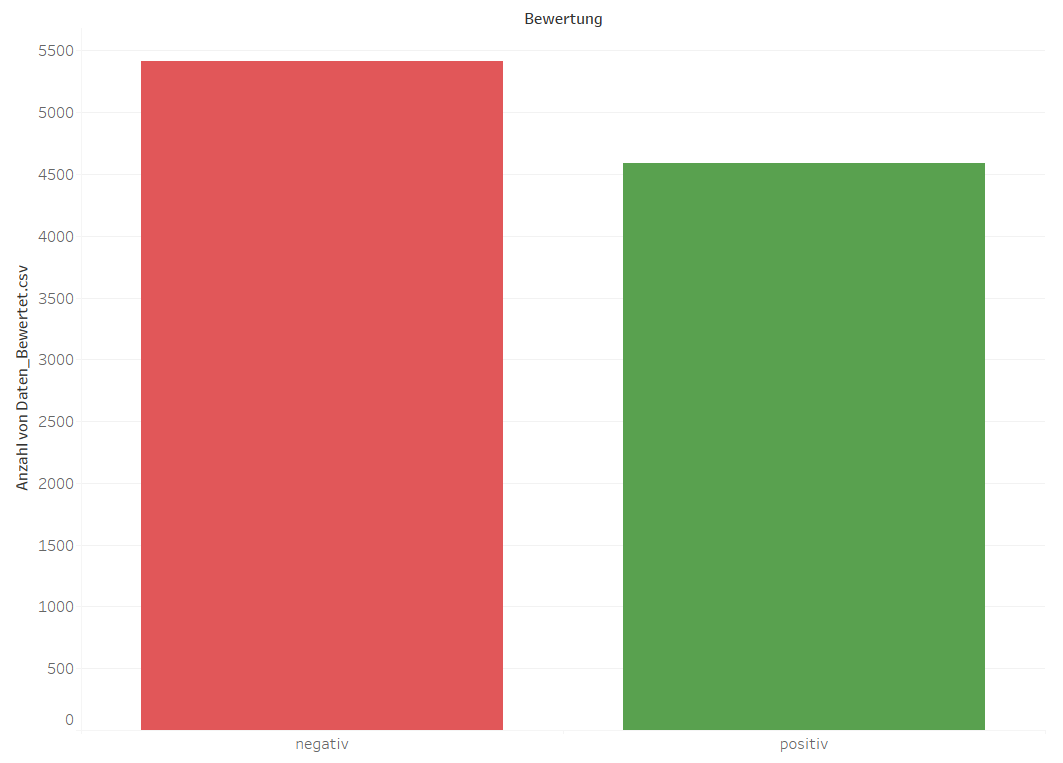
\includegraphics[width=16cm,height=12cm]{Diagramme/SZ1_Tab1.PNG}
    \caption{Überblick über die Verteilung der Bewertung}
    \label{fig:SZ1Tab1}
\end{figure}

\begin{figure}[!h]
    \centering
    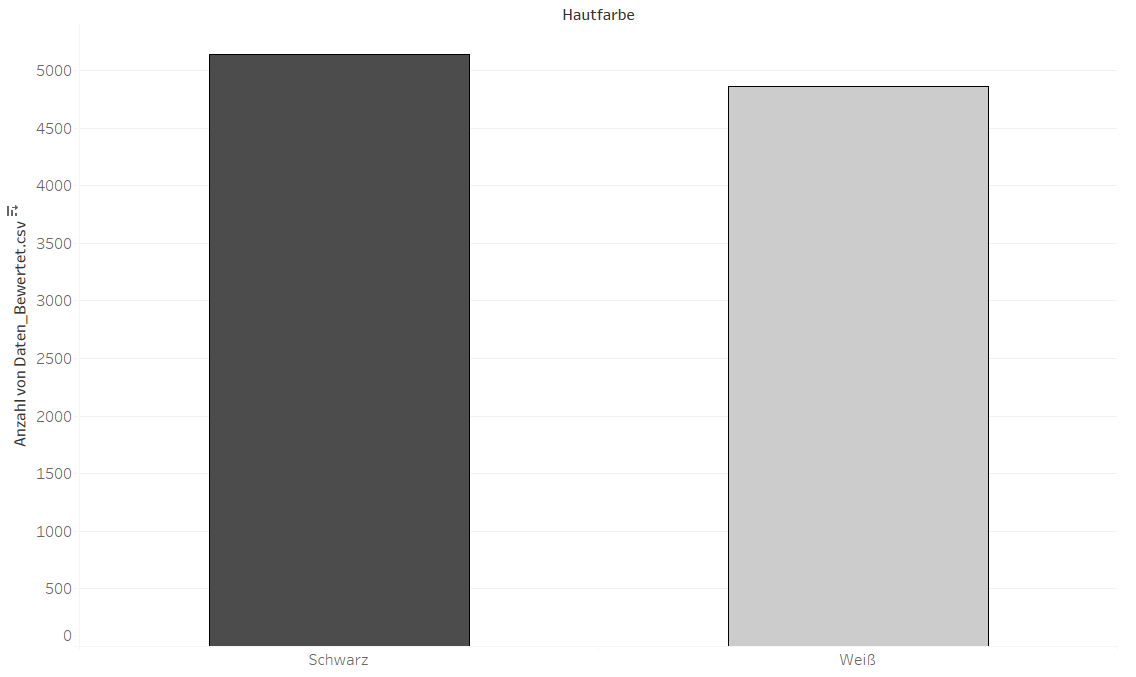
\includegraphics[width=16cm,height=12cm]{Diagramme/SZ1_Tab2.PNG}
    \caption{Überblick über die Verteilung der Hautfarbe}
    \label{fig:SZ1Tab2}
\end{figure}

\begin{figure}[!h]
    \centering
    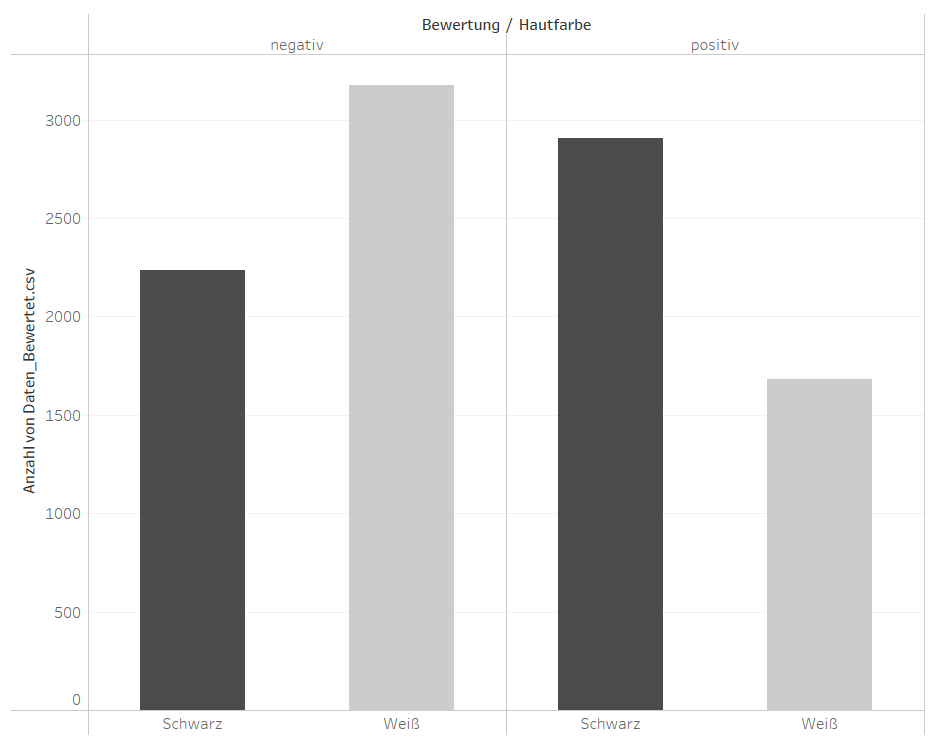
\includegraphics[width=16cm,height=12cm]{Diagramme/SZ1_Tab3.PNG}
    \caption{Auswertung der Hautfarbe im Zusammenhang mit der Bewertung nach Anzahl der gesamt Daten}
    \label{fig:SZ1Tab3}
\end{figure}

\begin{figure}[!h]
    \centering
    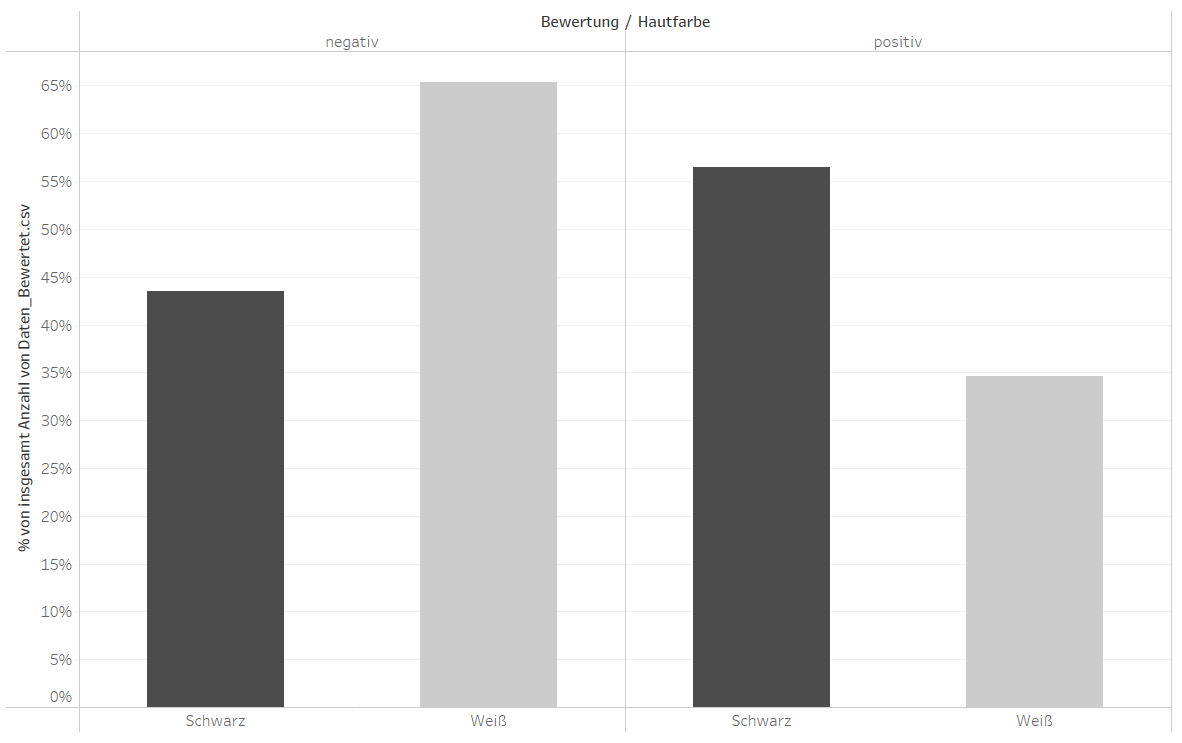
\includegraphics[width=16cm,height=12cm]{Diagramme/SZ1_Tab4.PNG}
    \caption{Auswertung der Hautfarbe im Zusammenhang mit der Bewertung nach Prozent von der gesamt Anzahl an Daten}
    \label{fig:SZ1Tab4}
\end{figure}

\begin{figure}[!h]
    \centering
    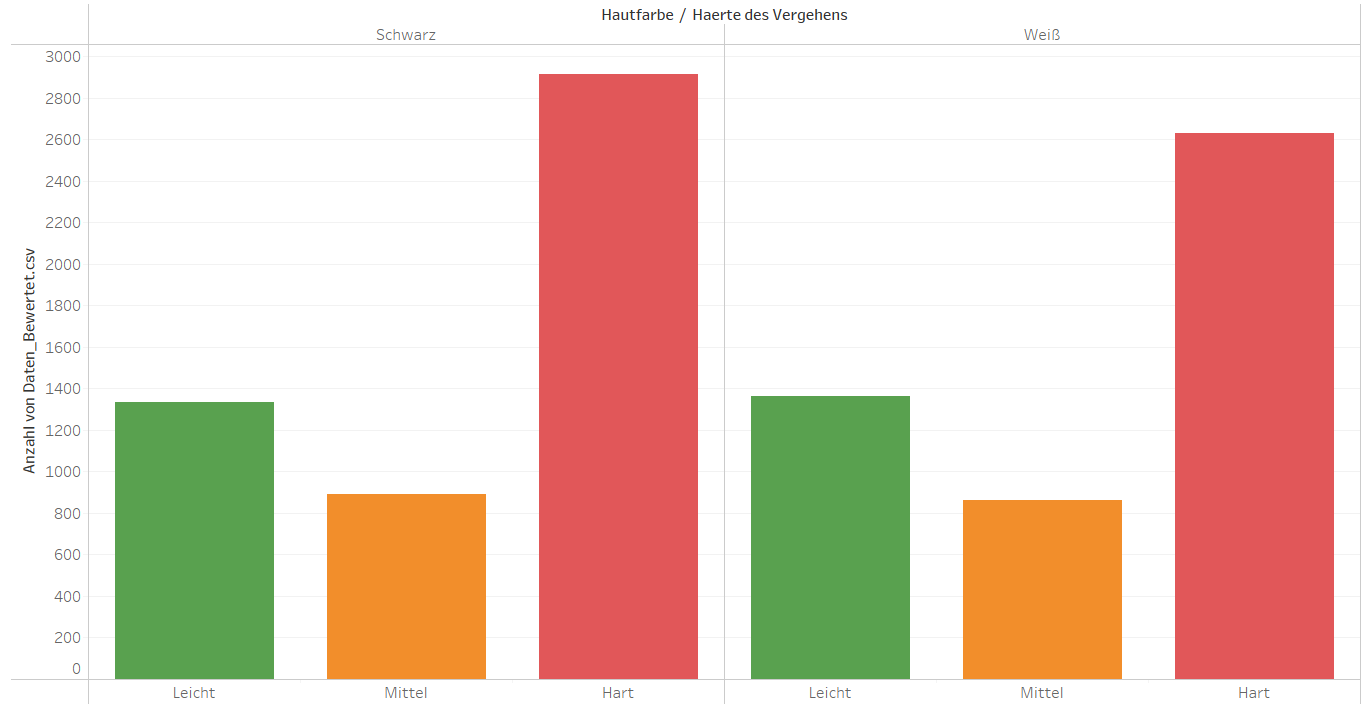
\includegraphics[width=16cm,height=12cm]{Diagramme/SZ1_Tab5.PNG}
    \caption{Auswertung der Hautfarbe im Zusammenhang mit der Härte des Vergehens nach Anzahl der gesamt Daten}
    \label{fig:SZ1Tab5}
\end{figure}

\begin{figure}[!h]
    \centering
    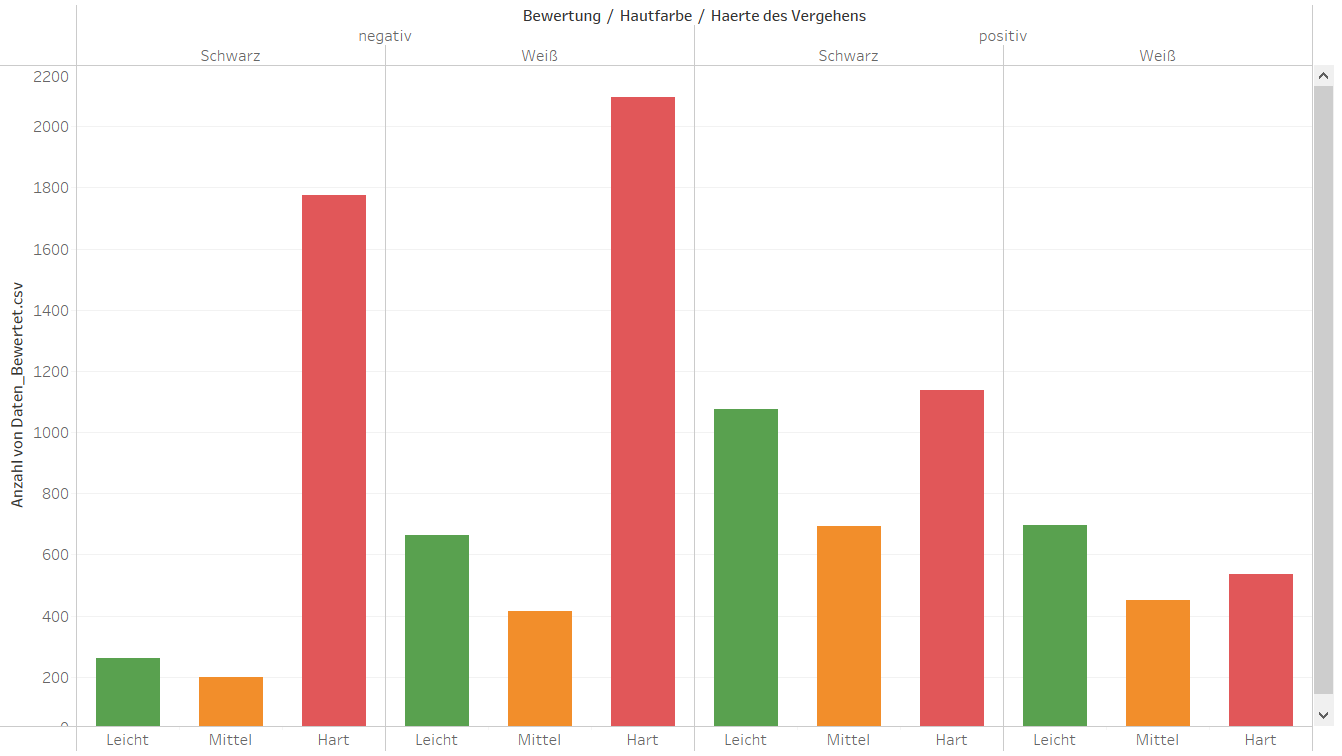
\includegraphics[width=16cm,height=12cm]{Diagramme/SZ1_Tab6.PNG}
    \caption{Auswertung der Hautfarbe im Zusammenhang mit der Härte der Strafe und der Bewertung nach der gesamt Anzahl an Daten}
    \label{fig:SZ1Tab6}
\end{figure}

\begin{figure}[!h]
    \centering
    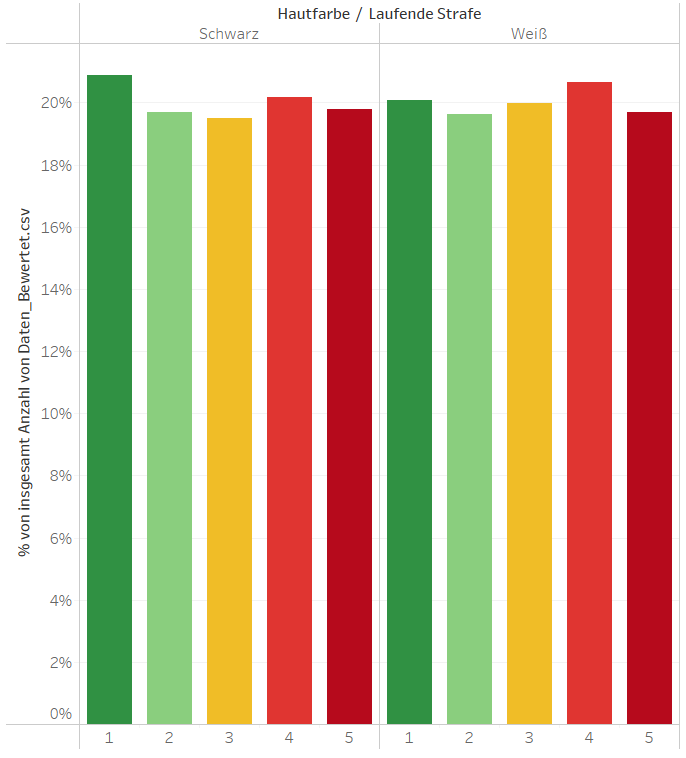
\includegraphics[width=16cm,height=12cm]{Diagramme/SZ1_Tab7.PNG}
    \caption{Auswertung der Hautfarbe im Zusammenhang mit der Laufenden Strafe nach Prozent von der gesamt Anzahl an Daten}
    \label{fig:SZ1Tab7}
\end{figure}

\begin{figure}[!h]
    \centering
    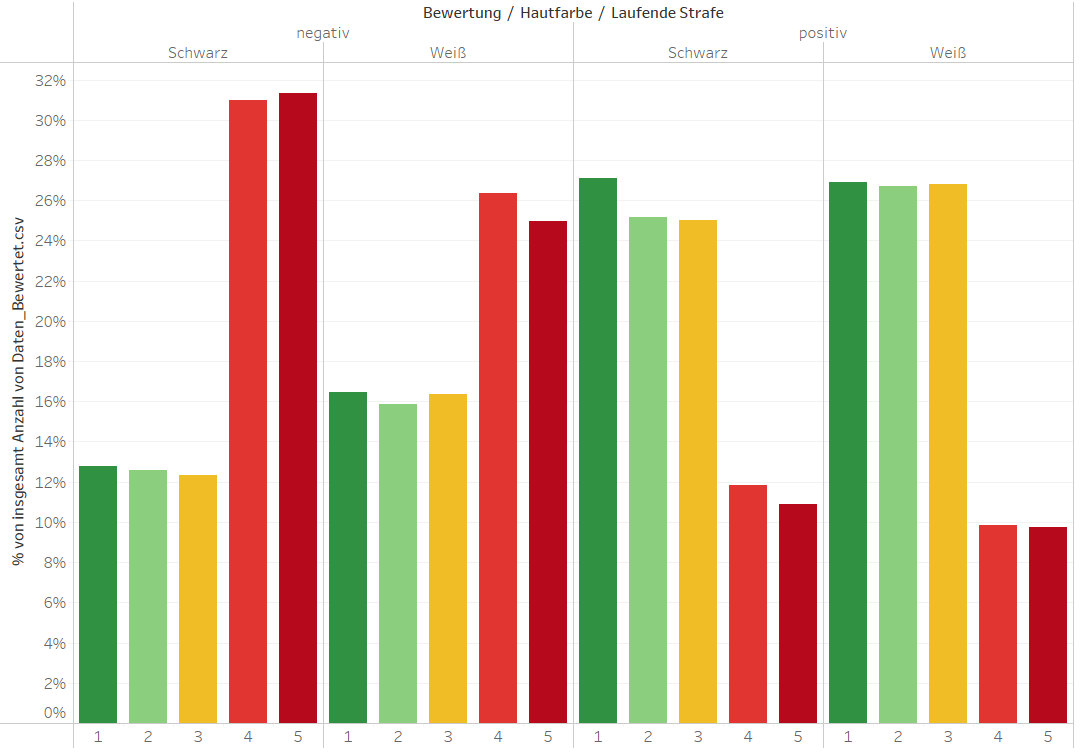
\includegraphics[width=16cm,height=12cm]{Diagramme/SZ1_Tab8.PNG}
    \caption{Auswertung der Hautfarbe im Zusammenhang mit der Laufenden Strafe und der Bewertung nach Prozent von der gesamt Anzahl an Daten}
    \label{fig:SZ1Tab8}
\end{figure}

\begin{figure}[!h]
    \centering
    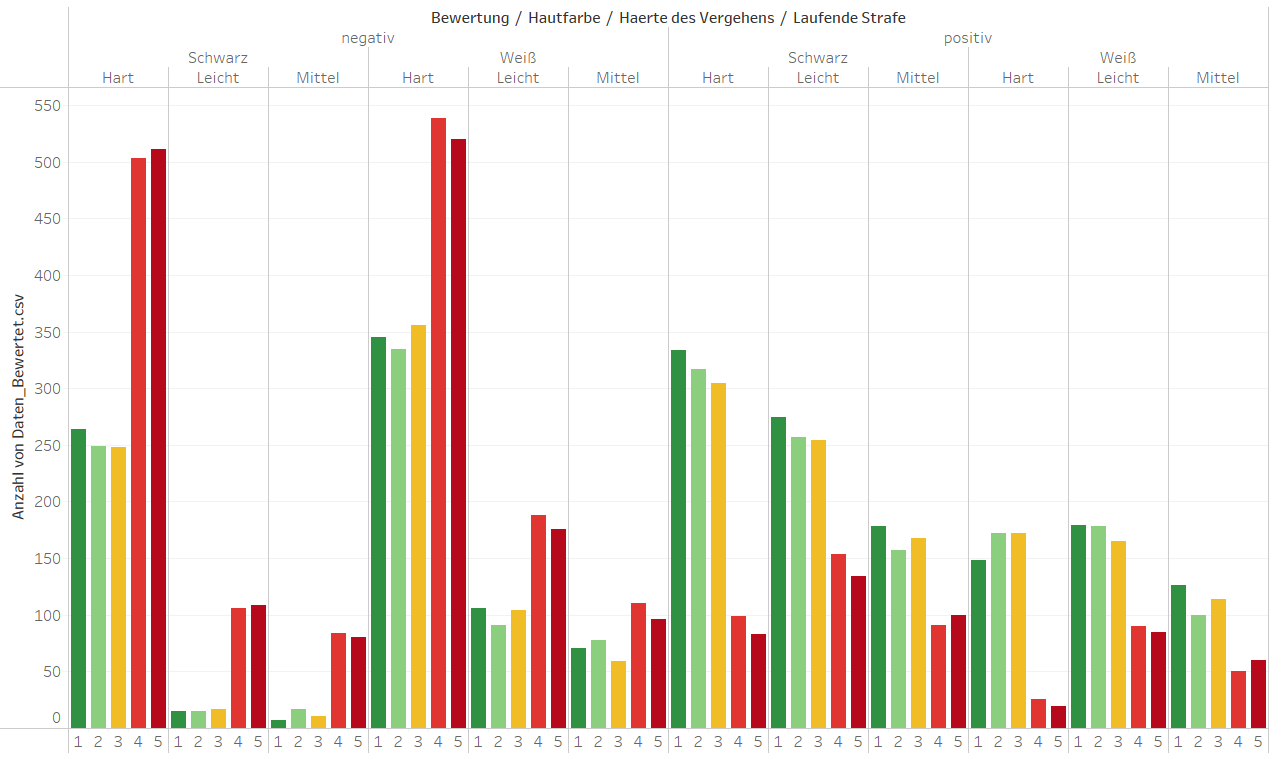
\includegraphics[width=16cm,height=12cm]{Diagramme/SZ1_Tab9.PNG}
    \caption{Auswertung der Hautfarbe im Zusammenhang mit der Bewertung, Härte der Strafe und Laufenden Strafe nach der gesamt Anzahl an Daten}
    \label{fig:SZ1Tab9}
\end{figure}

\begin{figure}[!h]
    \centering
    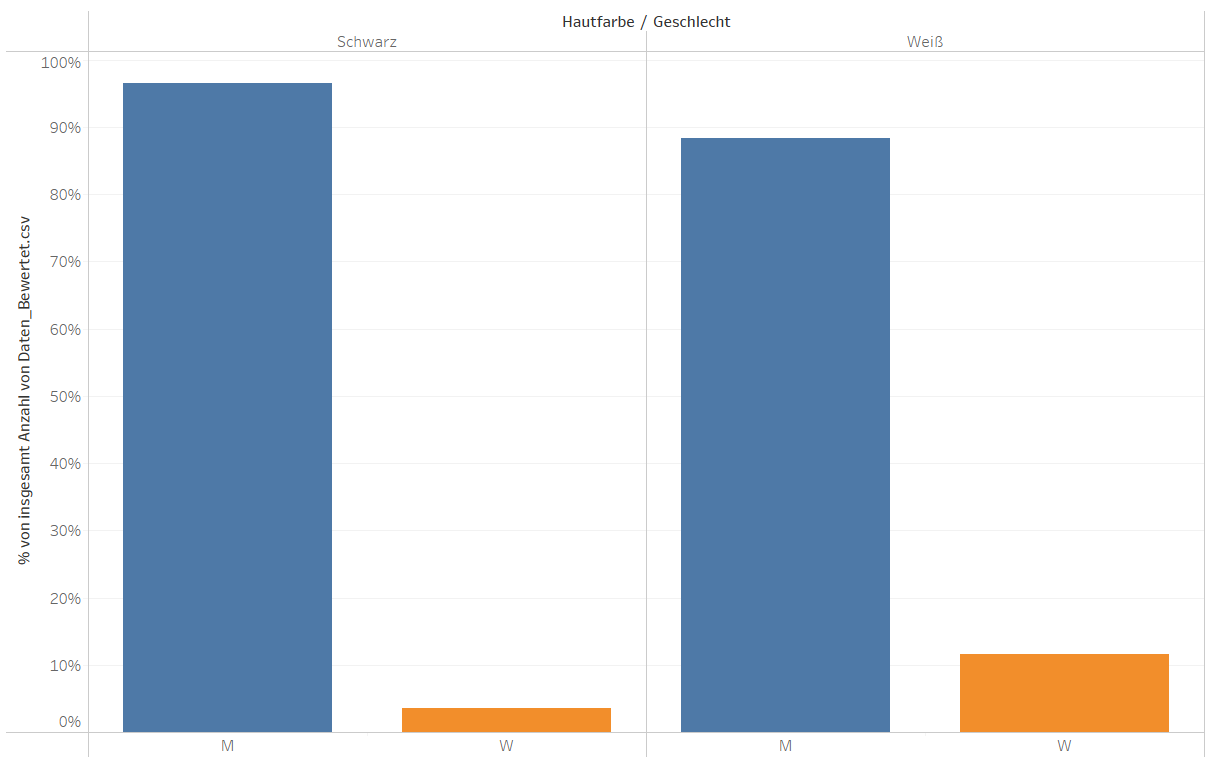
\includegraphics[width=16cm,height=12cm]{Diagramme/SZ1_Tab10.PNG}
    \caption{Verteilung des Geschlechts über die Hautfarbe}
    \label{fig:SZ1Tab10}
\end{figure}

    \chapter{Tableau für das Szenario zur Vorhersage eines sozialen Punktesystems}

\begin{figure}[!h]
    \centering
    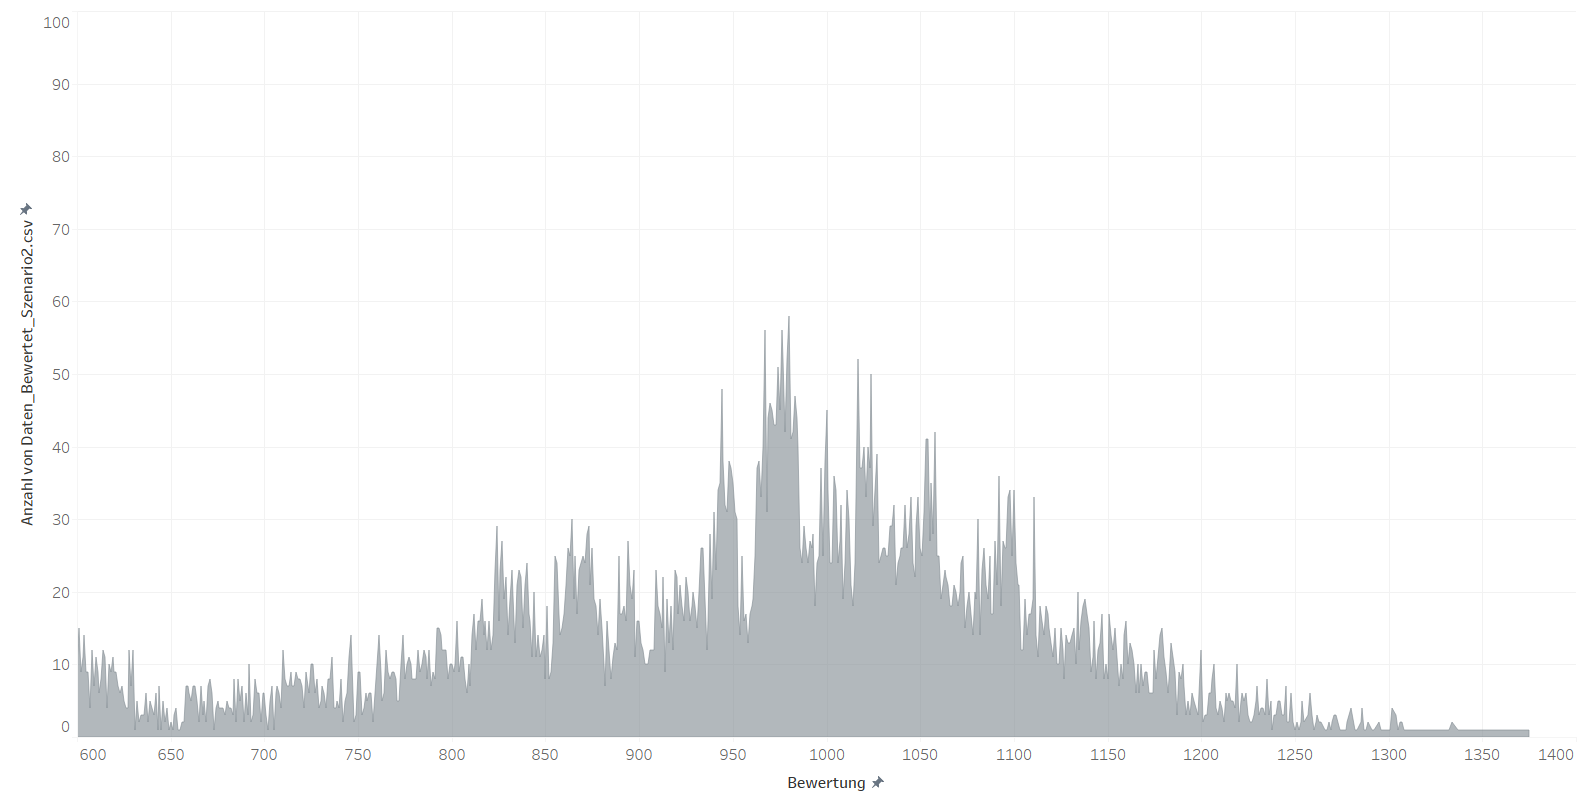
\includegraphics[width=16cm,height=12cm]{Diagramme/SZ2_Tab1.PNG}
    \caption{Überblick über die Verteilung der Bewertung}
    \label{fig:SZ2Tab1}
\end{figure}

\begin{figure}[!h]
    \centering
    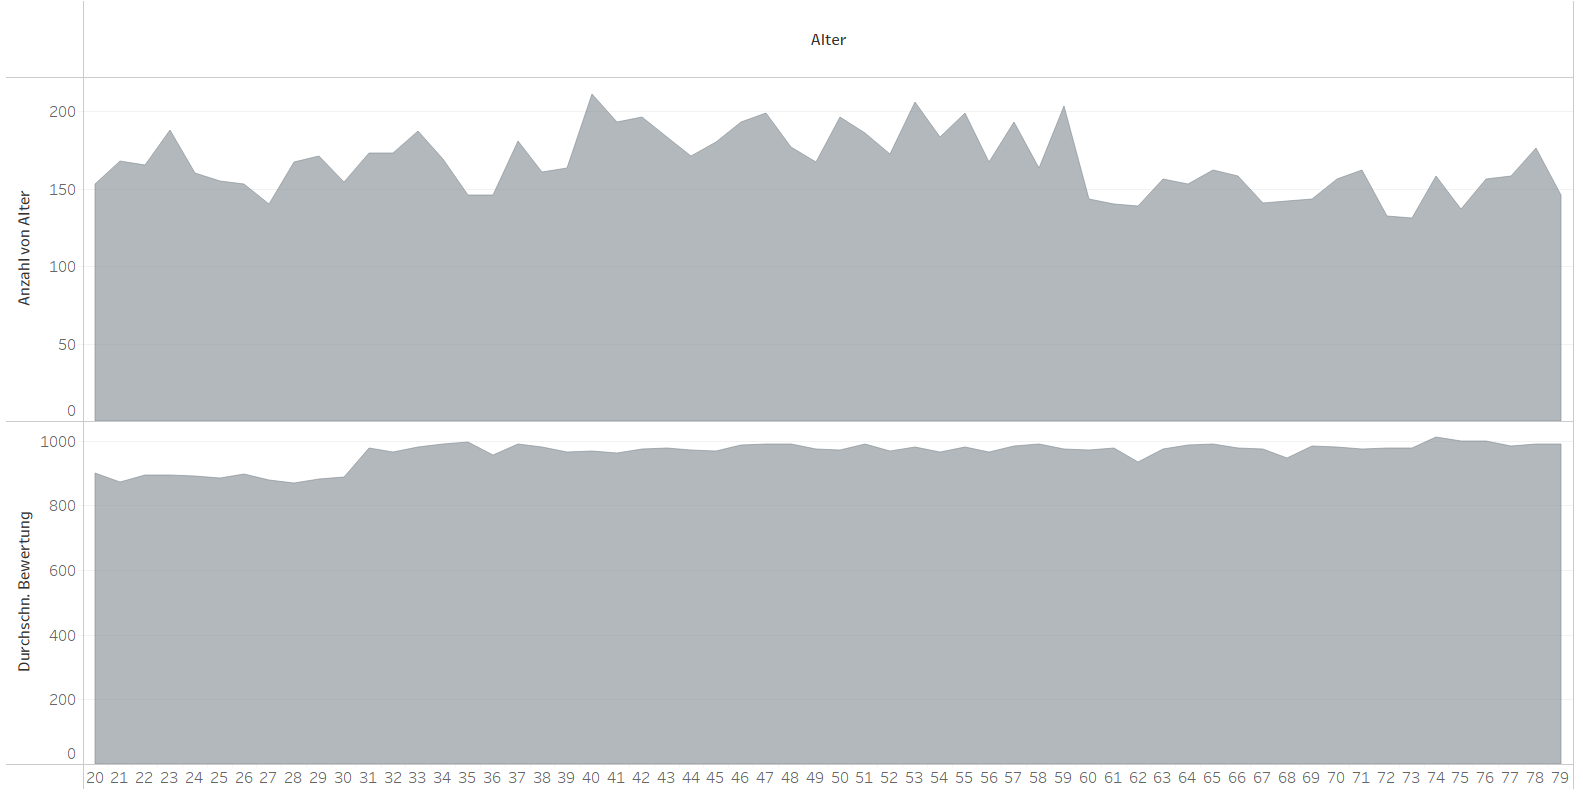
\includegraphics[width=16cm,height=12cm]{Diagramme/SZ2_Tab2.PNG}
    \caption{Auswertung der Anzahl von Personen und durchschnittlicher Punktestand pro Alter}
    \label{fig:SZ2Tab2}
\end{figure}

\begin{figure}[!h]
    \centering
    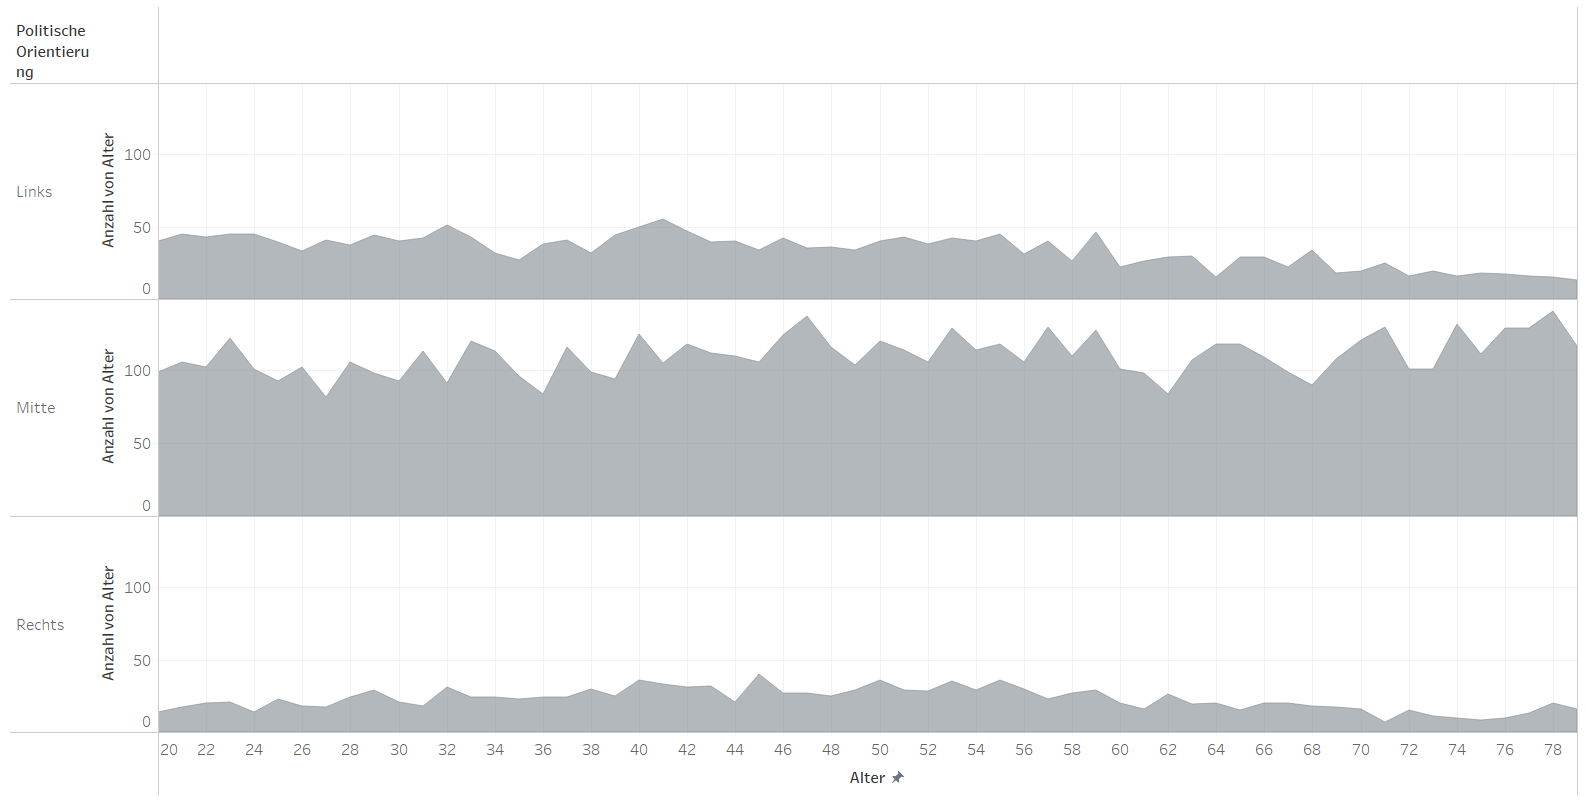
\includegraphics[width=16cm,height=12cm]{Diagramme/SZ2_Tab3.PNG}
    \caption{Auswertung der Anzahl von Personen pro Alter und politische Orientierung}
    \label{fig:SZ2Tab3}
\end{figure}

\begin{figure}[!h]
    \centering
    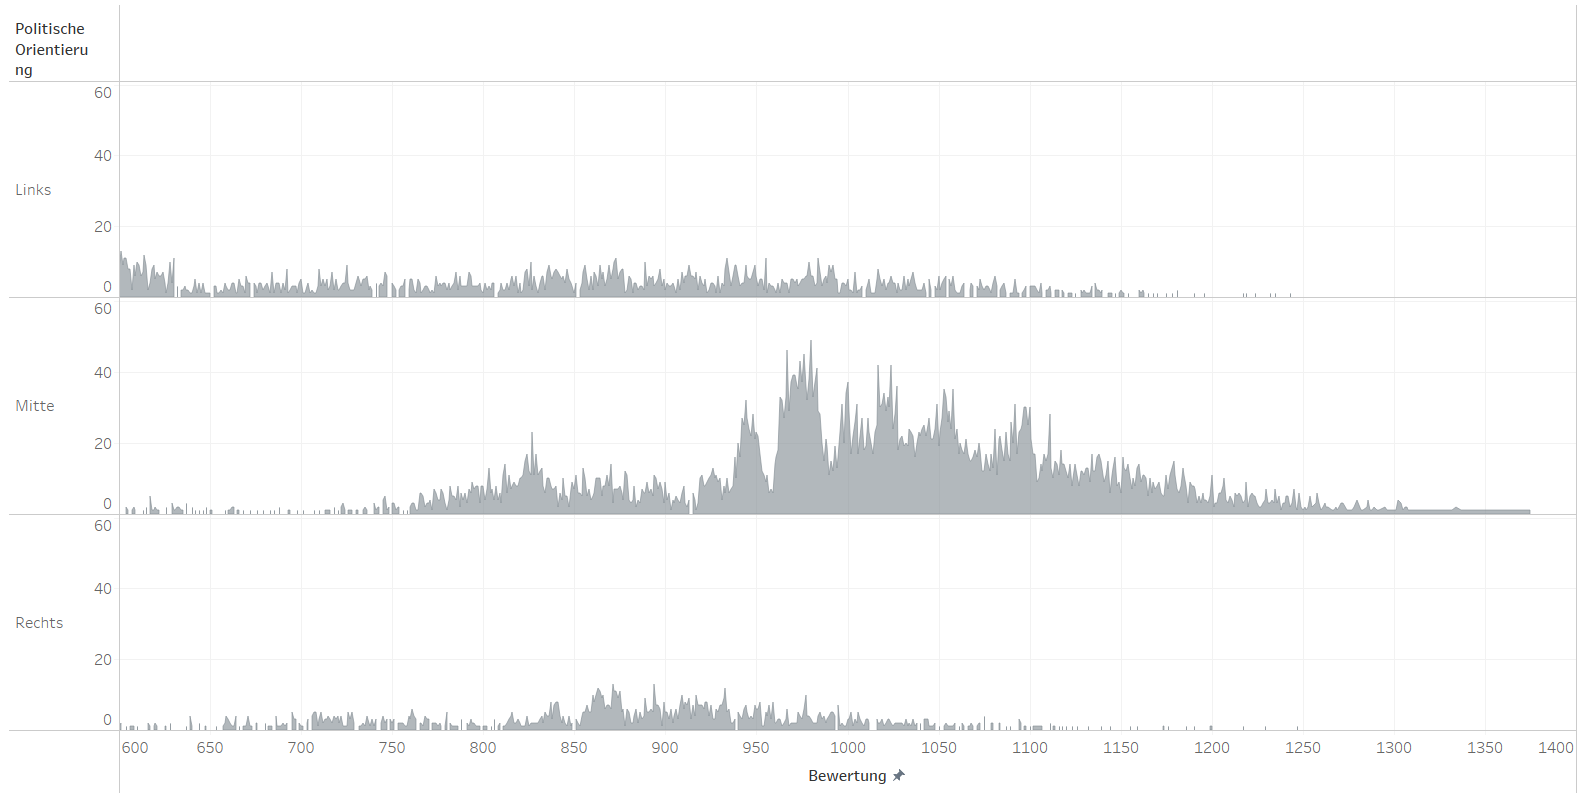
\includegraphics[width=16cm,height=12cm]{Diagramme/SZ2_Tab4.PNG}
    \caption{Auswertung des Punktestand pro politische Orientierung über alle Datenpunkte}
    \label{fig:SZ2Tab4}
\end{figure}

\begin{figure}[!h]
    \centering
    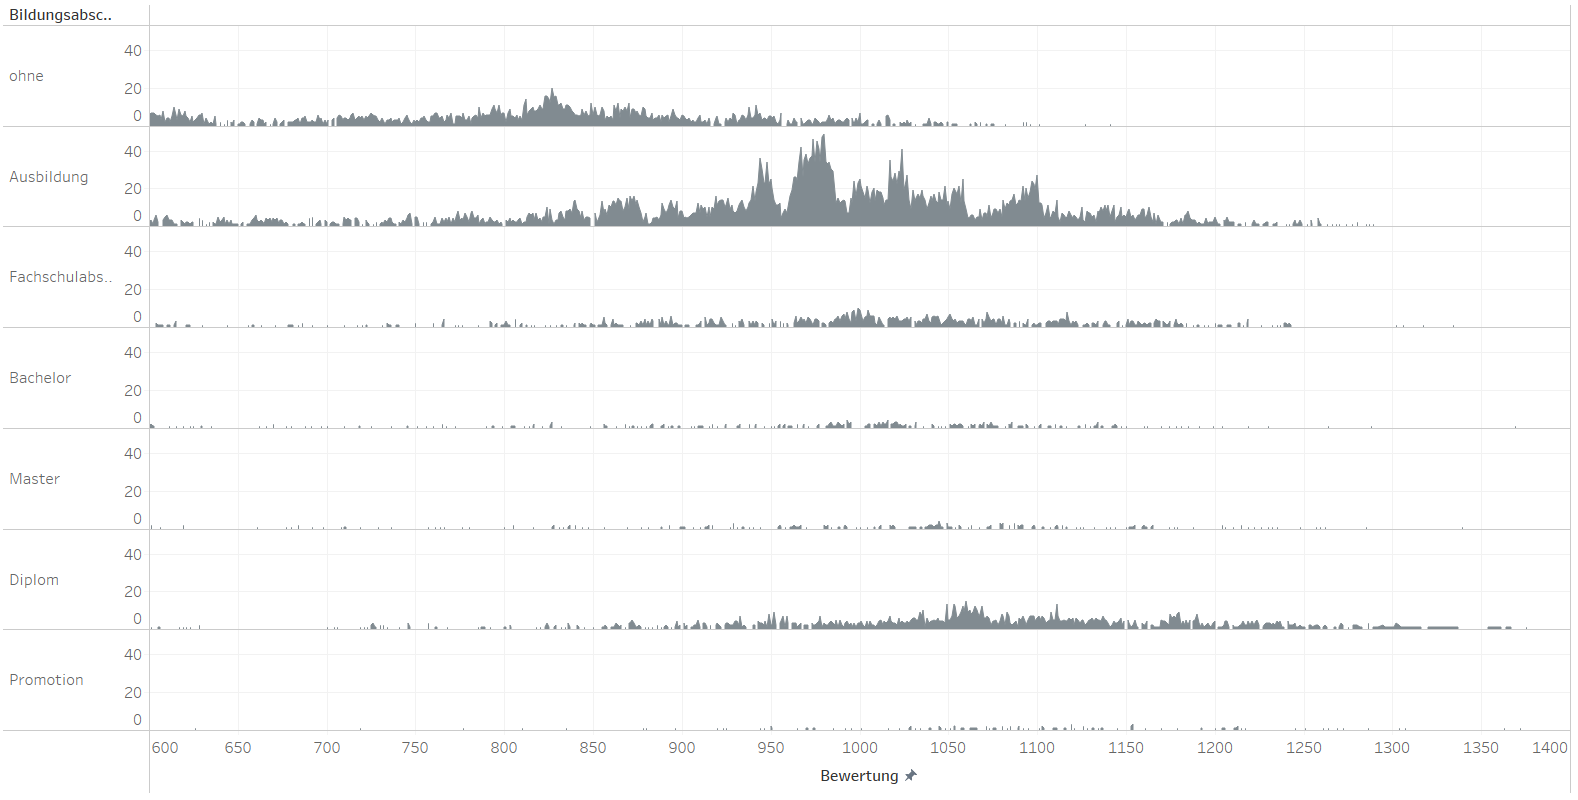
\includegraphics[width=16cm,height=12cm]{Diagramme/SZ2_Tab5.PNG}
    \caption{Auswertung des Punktestand für jeden Bildungsabschluss über alle Datenpunkte}
    \label{fig:SZ2Tab5}
\end{figure}

\begin{figure}[!h]
    \centering
    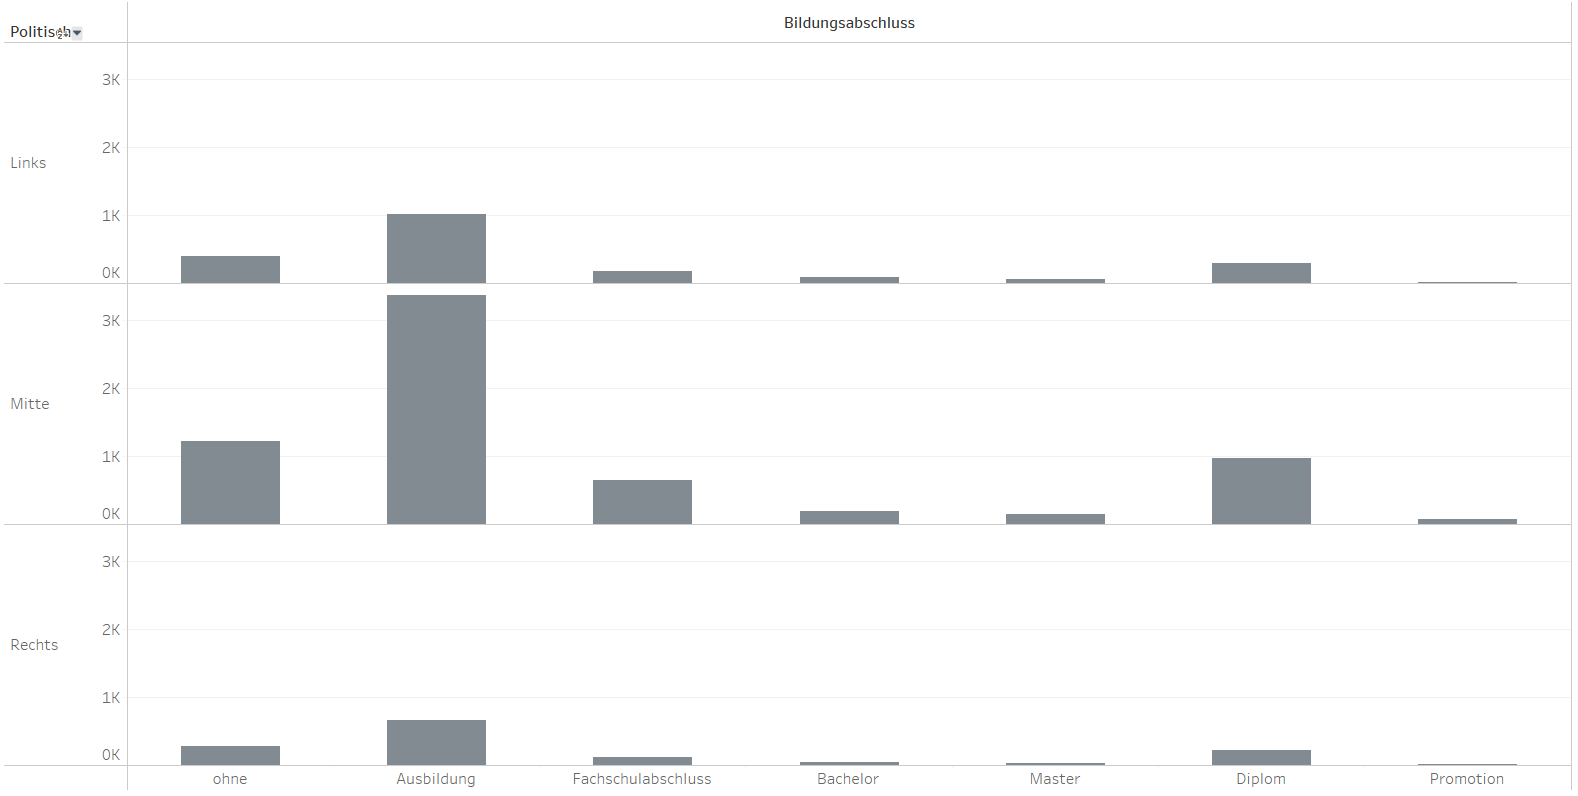
\includegraphics[width=16cm,height=12cm]{Diagramme/SZ2_Tab6.PNG}
    \caption{Auswertung der Anzahl an Datenpunkten für jeden Bildungsabschluss und jede politische Orientierung}
    \label{fig:SZ2Tab6}
\end{figure}

\begin{figure}[!h]
    \centering
    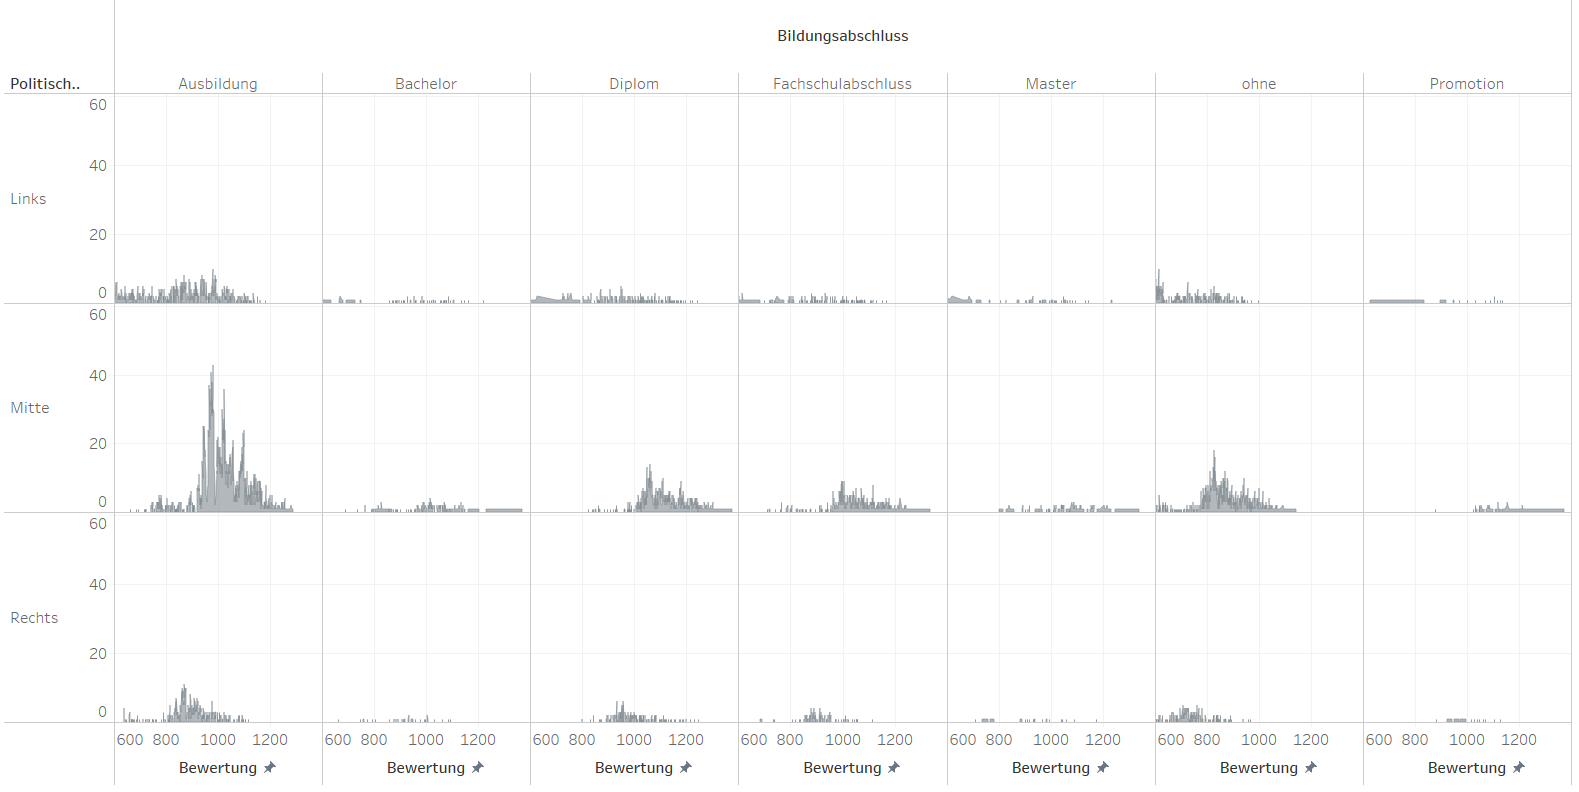
\includegraphics[width=16cm,height=12cm]{Diagramme/SZ2_Tab7.PNG}
    \caption{Auswertung des Punktestand für jeden Bildungsabschluss und politische Orientierung über alle Datenpunkte}
    \label{fig:SZ2Tab7}
\end{figure}

\begin{figure}[!h]
    \centering
    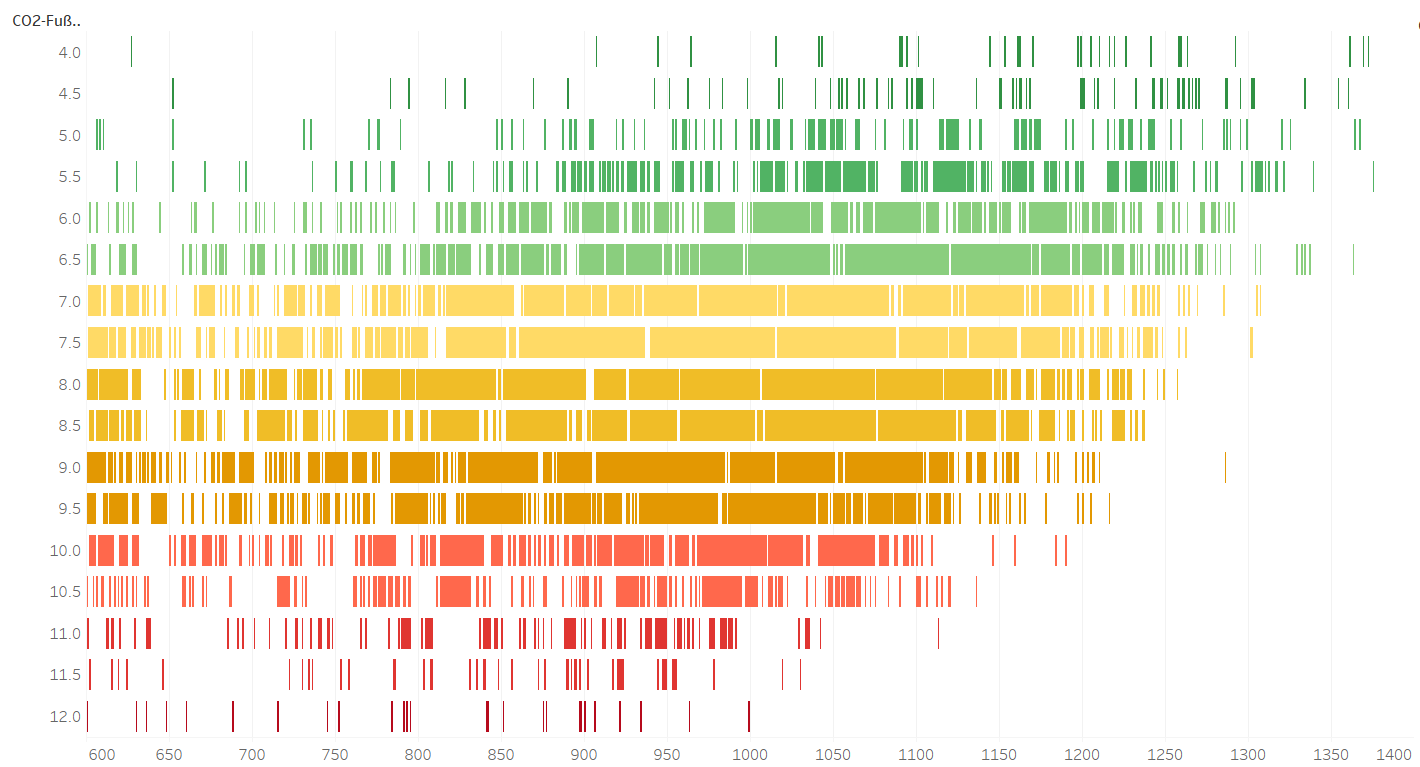
\includegraphics[width=16cm,height=12cm]{Diagramme/SZ2_Tab8.PNG}
    \caption{Auswertung des Punktestand für den CO2-Fußabdruck über alle Datenpunkte}
    \label{fig:SZ2Tab8}
\end{figure}

\begin{figure}[!h]
    \centering
    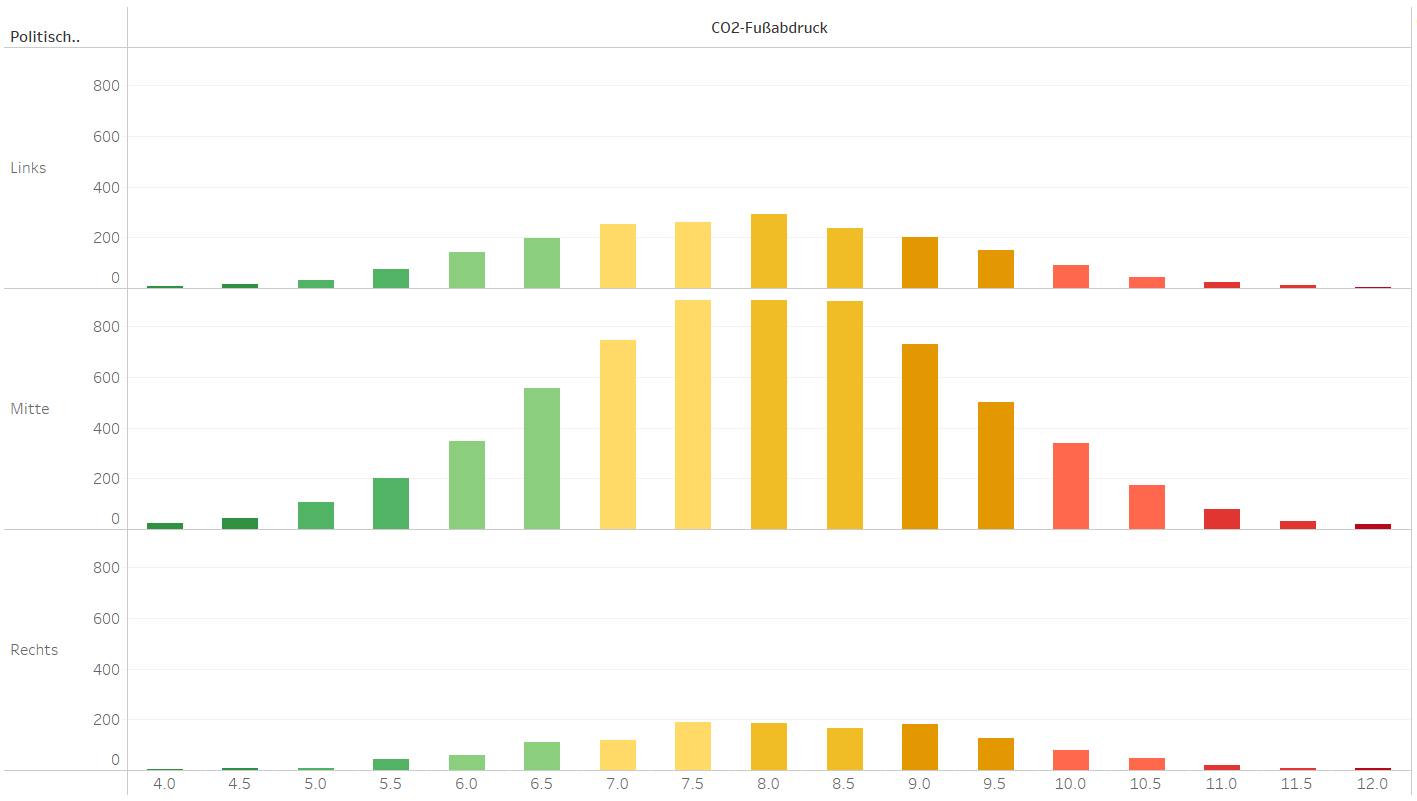
\includegraphics[width=16cm,height=12cm]{Diagramme/SZ2_Tab9.PNG}
    \caption{Auswertung der Anzahl an Datenpunkten für den CO2-Fußabdruck pro politische Orientierung}
    \label{fig:SZ2Tab9}
\end{figure}

\begin{figure}[!h]
    \centering
    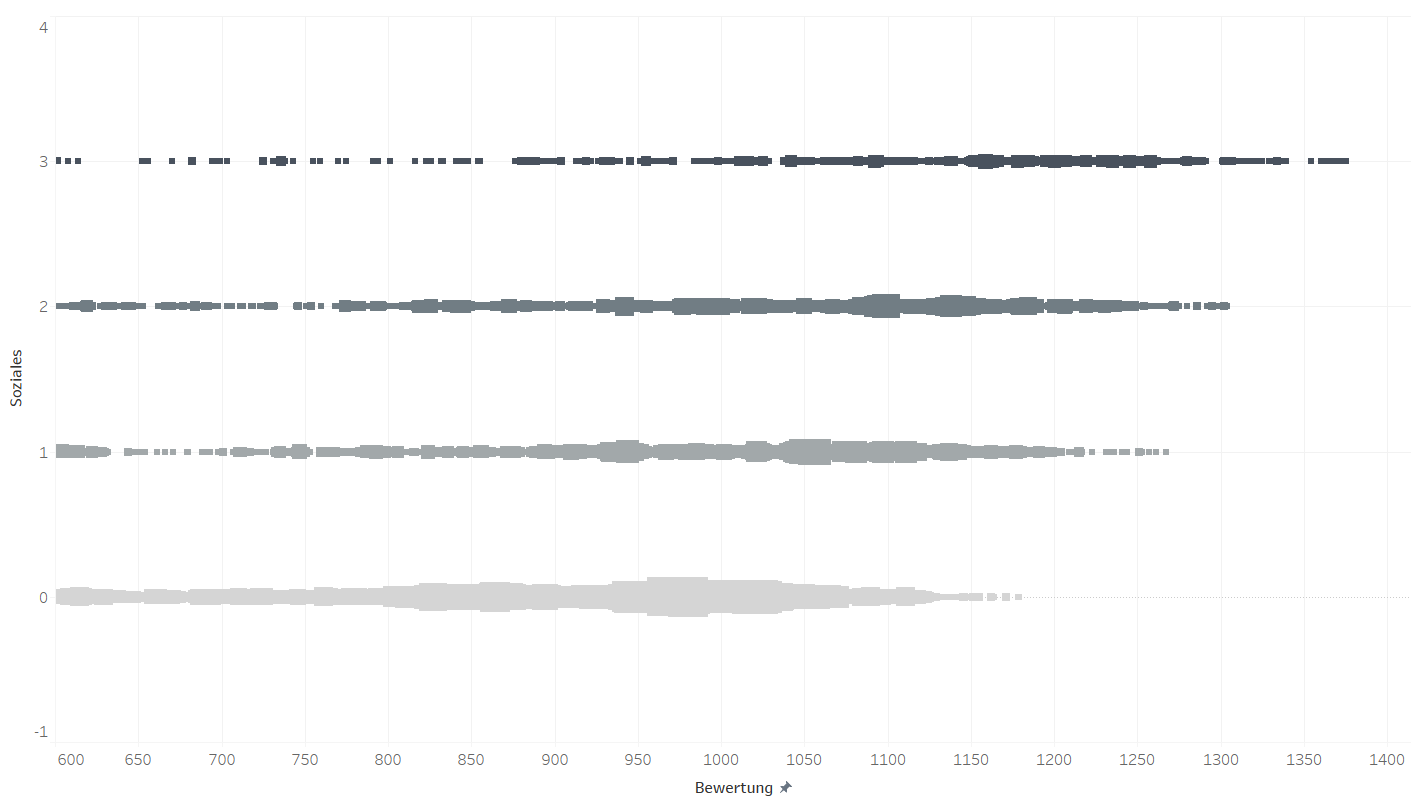
\includegraphics[width=16cm,height=12cm]{Diagramme/SZ2_Tab10.PNG}
    \caption{Auswertung des Punktestand für das soziale Engagement über alle Datenpunkte}
    \label{fig:SZ2Tab10}
\end{figure}

\begin{figure}[!h]
    \centering
    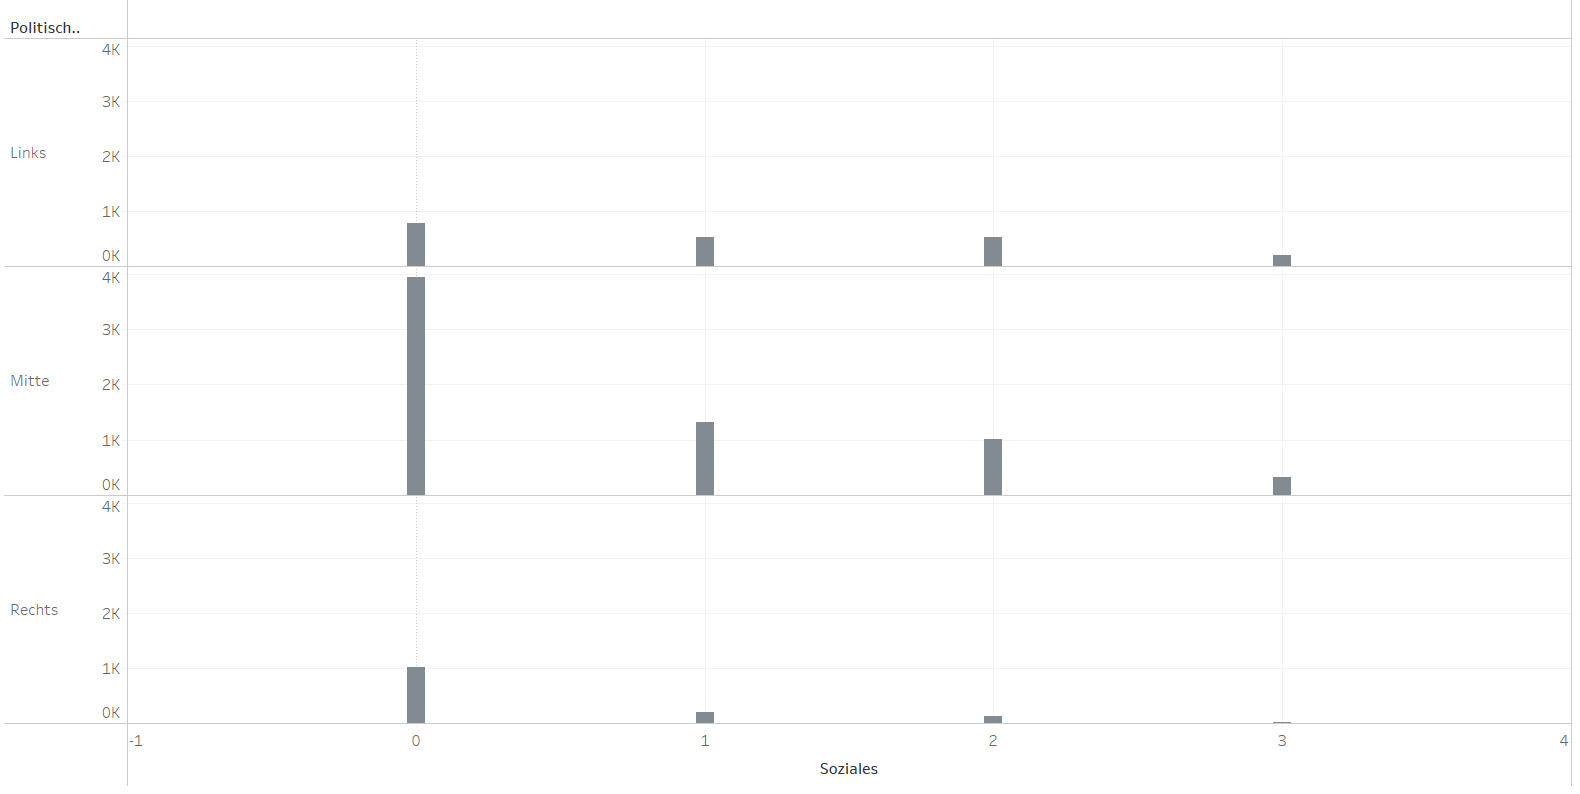
\includegraphics[width=16cm,height=12cm]{Diagramme/SZ2_Tab11.PNG}
    \caption{Auswertung der Anzahl an Datenpunkten für das soziale Engagement pro politische Orientierung}
    \label{fig:SZ2Tab11}
\end{figure}

\begin{figure}[!h]
    \centering
    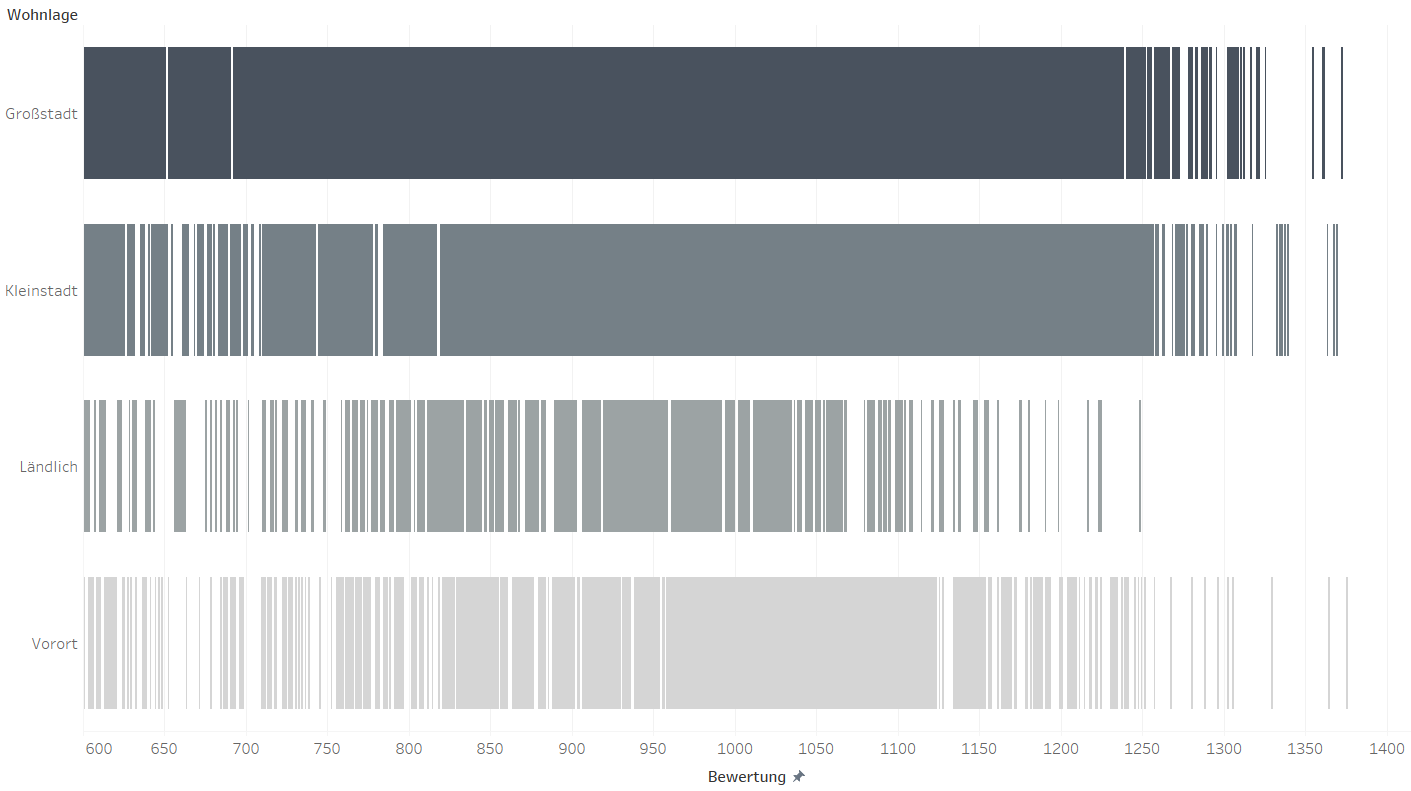
\includegraphics[width=16cm,height=12cm]{Diagramme/SZ2_Tab12.PNG}
    \caption{Auswertung des Punktestand für die Wohnlage über alle Datenpunkte}
    \label{fig:SZ2Tab12}
\end{figure}

\end{document}